%%%%%%%%%%%%%%%%%%%%%%%%%%%%%%%%%%%%%%%%%%%%%%%
%
% Template per Elaborato di Laurea
% DISI - Dipartimento di Ingegneria e Scienza dell’Informazione
%
% update 2015-09-10
%
% Per la generazione corretta del 
% pdflatex nome_file.tex
% bibtex nome_file.aux
% pdflatex nome_file.tex
% pdflatex nome_file.tex
%
%%%%%%%%%%%%%%%%%%%%%%%%%%%%%%%%%%%%%%%%%%%%%%%

% formato FRONTE RETRO
\documentclass[epsfig,a4paper,11pt,titlepage,twoside,openany]{book}
\usepackage{epsfig}
\usepackage{plain}
\usepackage{setspace}
\usepackage[paperheight=29.7cm,paperwidth=21cm,outer=1.5cm,inner=2.5cm,top=2cm,bottom=2cm]{geometry} % per definizione layout
\usepackage{titlesec} % per formato custom dei titoli dei capitoli

%%%%%%%%%%%%%%
% supporto lettere accentate
%
%\usepackage[latin1]{inputenc} % per Windows;
\usepackage[utf8x]{inputenc} % per Linux (richiede il pacchetto unicode);
%\usepackage[applemac]{inputenc} % per Mac.

\singlespacing

\usepackage[italian]{babel}

\begin{document}

  % nessuna numerazione
  \pagenumbering{gobble} 
  \pagestyle{plain}

\thispagestyle{empty}

\begin{center}
  \begin{figure}[h!]
    \centerline{
\psfig{file=marchio_unitrento_colore_it_v2.eps,width=0.6\textwidth}}
  \end{figure}

  \vspace{2 cm} 

  \LARGE{Department of Information Engineering and Computer Science\\}

  \vspace{1 cm} 
  \Large{Bachelor's degree in\\
    Computer Science
    %Informatica

  }

  \vspace{2 cm} 
  \Large\textsc{Final Dissertation\\} 
  \vspace{1 cm} 
  \Huge\textsc{INTERACTIVE DASHBOARDS FOR MEASURING WIKIPEDIA COMMUNITY HEALTH\\}
  
 \Large{\it{Technologies, contextualization and implementation of the Community Health Metrics dashboards}}


  \vspace{2 cm} 
  \begin{tabular*}{\textwidth}{ c @{\extracolsep{\fill}} c @{\extracolsep{\fill}} c }
  \vspace{.3 cm} 
  \Large{Supervisor} & \Large{Co-Supervisor} & \Large{Student}\\
  \vspace{.3 cm} 
  \Large{Alberto Montresor} & \Large{Cristian Consonni} & \Large{Paolo Aliprandi}\\
  \vspace{.3 cm} 
   & \Large{Marc Miquel-Ribé} & \\
   & \Large{David Laniado} & \\
  \end{tabular*}

  \vspace{2 cm} 

  \Large{Academic year 2021/2022}
  
\end{center}



  \clearpage
 
%%%%%%%%%%%%%%%%%%%%%%%%%%%%%%%%%%%%%%%%%%%%%%%%%%%%%%%%%%%%%%%%%%%%%%%%%%
%%%%%%%%%%%%%%%%%%%%%%%%%%%%%%%%%%%%%%%%%%%%%%%%%%%%%%%%%%%%%%%%%%%%%%%%%%
%% Nota
%%%%%%%%%%%%%%%%%%%%%%%%%%%%%%%%%%%%%%%%%%%%%%%%%%%%%%%%%%%%%%%%%%%%%%%%%%
%% Sezione Ringraziamenti opzionale
%%%%%%%%%%%%%%%%%%%%%%%%%%%%%%%%%%%%%%%%%%%%%%%%%%%%%%%%%%%%%%%%%%%%%%%%%%
%%%%%%%%%%%%%%%%%%%%%%%%%%%%%%%%%%%%%%%%%%%%%%%%%%%%%%%%%%%%%%%%%%%%%%%%%%
  \thispagestyle{empty}

\begin{center}
  {\bf \Huge Ringraziamenti}
\end{center}

\vspace{4cm}


\emph{
  ...thanks to...
}

  \clearpage
  \pagestyle{plain} % nessuna intestazione e pie pagina con numero al centro

  
  % inizio numerazione pagine in numeri arabi
  \mainmatter

%%%%%%%%%%%%%%%%%%%%%%%%%%%%%%%%%%%%%%%%%%%%%%%%%%%%%%%%%%%%%%%%%%%%%%%%%%
%%%%%%%%%%%%%%%%%%%%%%%%%%%%%%%%%%%%%%%%%%%%%%%%%%%%%%%%%%%%%%%%%%%%%%%%%%
%% Nota
%%%%%%%%%%%%%%%%%%%%%%%%%%%%%%%%%%%%%%%%%%%%%%%%%%%%%%%%%%%%%%%%%%%%%%%%%%
%% Si ricorda che il numero massimo di facciate e' 30.
%% Nel conteggio delle facciate sono incluse 
%%   indice
%%   sommario
%%   capitoli
%% Dal conteggio delle facciate sono escluse
%%   frontespizio
%%   ringraziamenti
%%   allegati    
%%%%%%%%%%%%%%%%%%%%%%%%%%%%%%%%%%%%%%%%%%%%%%%%%%%%%%%%%%%%%%%%%%%%%%%%%%
%%%%%%%%%%%%%%%%%%%%%%%%%%%%%%%%%%%%%%%%%%%%%%%%%%%%%%%%%%%%%%%%%%%%%%%%%%

    % indice
    \tableofcontents
    \clearpage
    
    
          
    % gruppo per definizone di successione capitoli senza interruzione di pagina
    \begingroup
      % nessuna interruzione di pagina tra capitoli
      % ridefinizione dei comandi di clear page
      \renewcommand{\cleardoublepage}{} 
      \renewcommand{\clearpage}{} 
      % redefinizione del formato del titolo del capitolo
      % da formato
      %   Capitolo X
      %   Titolo capitolo
      % a formato
      %   X   Titolo capitolo
      
      \titleformat{\chapter}
        {\normalfont\Huge\bfseries}{\thechapter}{1em}{}
        
      \titlespacing*{\chapter}{0pt}{0.59in}{0.02in}
      \titlespacing*{\section}{0pt}{0.20in}{0.02in}
      \titlespacing*{\subsection}{0pt}{0.10in}{0.02in}
      
      % sommario
      \chapter*{Sommario} % senza numerazione
\label{sommario}

\addcontentsline{toc}{chapter}{Sommario} % da aggiungere comunque all'indice

Lorem ipsum dolor sit amet, consectetur adipiscing elit. Donec sed nunc orci. Aliquam nec nisl vitae sapien pulvinar dictum quis non urna. Suspendisse at dui a erat aliquam vestibulum. Quisque ultrices pellentesque pellentesque. Pellentesque egestas quam sed blandit tempus. Sed congue nec risus posuere euismod. Maecenas ut lacus id mauris sagittis egestas a eu dui. Class aptent taciti sociosqu ad litora torquent per conubia nostra, per inceptos himenaeos. Pellentesque at ultrices tellus. Ut eu purus eget sem iaculis ultricies sed non lorem. Curabitur gravida dui eget ex vestibulum venenatis. Phasellus gravida tellus velit, non eleifend justo lobortis eget.


  Sommario è un breve riassunto del lavoro svolto dove si descrive l'obiettivo, l'oggetto della tesi, le 
metodologie e le tecniche usate, i dati elaborati e la spiegazione delle conclusioni alle quali siete arrivati.  

Il sommario dell’elaborato consiste al massimo di 3 pagine e deve contenere le seguenti informazioni:
\begin{itemize}
  \item contesto e motivazioni 
  \item breve riassunto del problema affrontato
  \item tecniche utilizzate e/o sviluppate
  \item risultati raggiunti, sottolineando il contributo personale del laureando/a
\end{itemize}





%%%%%%%%%%%%%%%%%%%%%%%%%%%%%%%%%%%%%%%%%%%%%%%%%%%%%%%%%%%%%%%%%%%%%%%%%%
%%%%%%%%%%%%%%%%%%%%%%%%%%%%%%%%%%%%%%%%%%%%%%%%%%%%%%%%%%%%%%%%%%%%%%%%%%
%% Nota
%%%%%%%%%%%%%%%%%%%%%%%%%%%%%%%%%%%%%%%%%%%%%%%%%%%%%%%%%%%%%%%%%%%%%%%%%%
%% Sommario e' un breve riassunto del lavoro svolto dove si descrive 
%% l’obiettivo, l’oggetto della tesi, le metodologie e 
%% le tecniche usate, i dati elaborati e la spiegazione delle conclusioni 
%% alle quali siete arrivati.
%% Il sommario dell’elaborato consiste al massimo di 3 pagine e deve contenere le seguenti informazioni: 
%%   contesto e motivazioni
%%   breve riassunto del problema affrontato
%%   tecniche utilizzate e/o sviluppate
%%   risultati raggiunti, sottolineando il contributo personale del laureando/a
%%%%%%%%%%%%%%%%%%%%%%%%%%%%%%%%%%%%%%%%%%%%%%%%%%%%%%%%%%%%%%%%%%%%%%%%%%
%%%%%%%%%%%%%%%%%%%%%%%%%%%%%%%%%%%%%%%%%%%%%%%%%%%%%%%%%%%%%%%%%%%%%%%%%%      
      
      %%%%%%%%%%%%%%%%%%%%%%%%%%%%%%%%
      % lista dei capitoli
      %
      % \input oppure \include
      %
      \chapter{In ante nulla, vestibulum a}
\label{cha:intro}

Lorem ipsum dolor sit amet, consectetur adipiscing elit. Donec sed nunc orci. Aliquam nec nisl vitae sapien pulvinar dictum quis non urna. Suspendisse at dui a erat aliquam vestibulum. Quisque ultrices pellentesque pellentesque. Pellentesque egestas quam sed blandit tempus. Sed congue nec risus posuere euismod. Maecenas ut lacus id mauris sagittis egestas a eu dui. Class aptent taciti sociosqu ad litora torquent per conubia nostra, per inceptos himenaeos. Pellentesque at ultrices tellus. Ut eu purus eget sem iaculis ultricies sed non lorem. Curabitur gravida dui eget ex vestibulum venenatis. Phasellus gravida tellus velit, non eleifend justo lobortis eget. 
\cite{coulouris}

Donec eu ipsum id lorem consectetur luctus ac a nisi. Curabitur volutpat, metus id porta ultrices, felis lacus consectetur justo, ut gravida arcu ex in purus. Pellentesque vitae sapien ac nisl porttitor pellentesque eu sed elit. Sed maximus lectus eu eros ultricies accumsan. Quisque congue, nisi in dictum cursus, ante nisl molestie eros, in ultrices eros tellus sit amet augue. Interdum et malesuada fames ac ante ipsum primis in faucibus. Nam finibus leo sit amet purus vehicula, eget facilisis turpis convallis. Vivamus varius tincidunt turpis, id venenatis arcu maximus ut. Aenean euismod eros ac nibh facilisis, nec imperdiet ex suscipit.
\cite{dalal}


\section{Pellentesque habitant morbi tristique senectus}
\label{sec:context}

Lorem ipsum dolor sit amet, consectetur adipiscing elit. Donec sed nunc orci. Aliquam nec nisl vitae sapien pulvinar dictum quis non urna. Suspendisse at dui a erat aliquam vestibulum. Quisque ultrices pellentesque pellentesque. Pellentesque egestas quam sed blandit tempus. Sed congue nec risus posuere euismod. Maecenas ut lacus id mauris sagittis egestas a eu dui. Class aptent taciti sociosqu ad litora torquent per conubia nostra, per inceptos himenaeos. Pellentesque at ultrices tellus. Ut eu purus eget sem iaculis ultricies sed non lorem. Curabitur gravida dui eget ex vestibulum venenatis. Phasellus gravida tellus velit, non eleifend justo lobortis eget.
\cite{ictbusiness}
\cite{donoho}

\section{Nullam et justo vitae nisi}
\label{sec:problem}

Lorem ipsum dolor sit amet, consectetur adipiscing elit. Donec sed nunc orci. Aliquam nec nisl vitae sapien pulvinar dictum quis non urna. Suspendisse at dui a erat aliquam vestibulum. Quisque ultrices pellentesque pellentesque. Pellentesque egestas quam sed blandit tempus. Sed congue nec risus posuere euismod. Maecenas ut lacus id mauris sagittis egestas a eu dui. Class aptent taciti sociosqu ad litora torquent per conubia nostra, per inceptos himenaeos. Pellentesque at ultrices tellus. Ut eu purus eget sem iaculis ultricies sed non lorem. Curabitur gravida dui eget ex vestibulum venenatis. Phasellus gravida tellus velit, non eleifend justo lobortis eget.



      \chapter{Technologies and Architecture}
\label{cha:456}
This chapter describes the Python modules used to build and run the Dashboards, and how they are structured.\\
The vital signs dashboards have been constructed as a dynamic website that allows user interaction.\\
Let us now describe the role of each Python module.

\section{Plotly}
\label{sec:plotly}
Plotly is a Python graphing library that provides a wide variety of charts for visualising data.
Since we get to plot different data, we need different charts to provide the best suited graph for each data we want to visualize. Each of them is interactive. \\
We remind that the goal of the project is to make the user understand what is going on with Wikipedia health metrics.\\
The power of Plotly is that it allows the graphs to change which data column to show, so the user has the possibility to see exactly the data he or she is interested in: from the time period to the value type.
To create the graphs we use two different sub-modules of Plotly:
\begin{itemize}
    \item \textbf{Graph objects \cite{go}:} The figures created, manipulated and rendered by this plotly Python library are represented by tree-like data structures which are automatically serialized to JSON. These trees are composed of named nodes called ``attributes''. The \verb#plotly.graph# objects module, imported as \verb#go#, contains an automatically-generated hierarchy of Python classes which represent non-leaf nodes in this figure schema. The term "graph objects" refers to instances of these classes.
    \item \textbf{Plotly express \cite{px}:} The Plotly express module, imported as \verb#px#, contains functions that can create entire figures at once. It is a built-in part of the Plotly library, and is the starting point for creating most common figures. Every Plotly Express function uses graph objects internally and returns a Plotly \verb#go.Figure# instance.
    The module \verb#px# was preferred due to its simplicity and more expressive syntax. 
\end{itemize}
In the visual dashboards, we find four different type of graphs:
\begin{figure}[!ht]
  \centering
  \setlocalecaption{english}{figure}{Figure}
  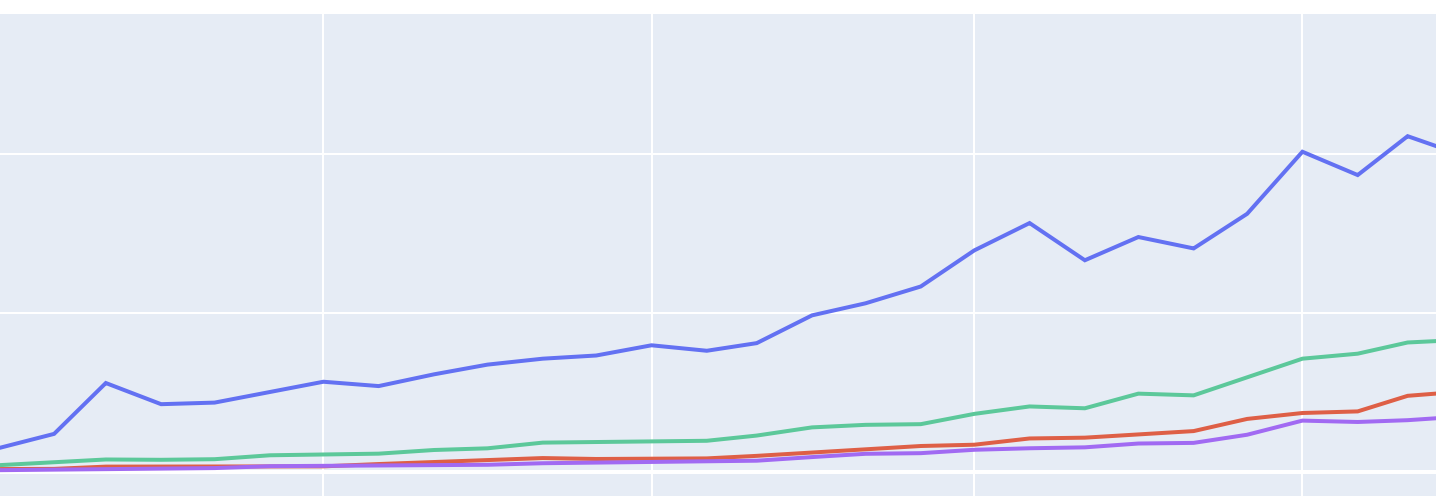
\includegraphics[width=5in]{img/line_chart.png}
  \caption{Line chart}
  \label{fig2.2}
\end{figure}
\\
\pagebreak
\paragraph{Line chart(Figure 2.1)}
We use them when we want to move the focus on the evolution of our data in time, especially when comparing different classes of data.\\
In this example we can see the evolution in time of the number of active editors of different language communities. In the next chapter we will focus more on this concept.
\\
\begin{figure}[!ht]
  \centering
  \setlocalecaption{english}{figure}{Figure}
  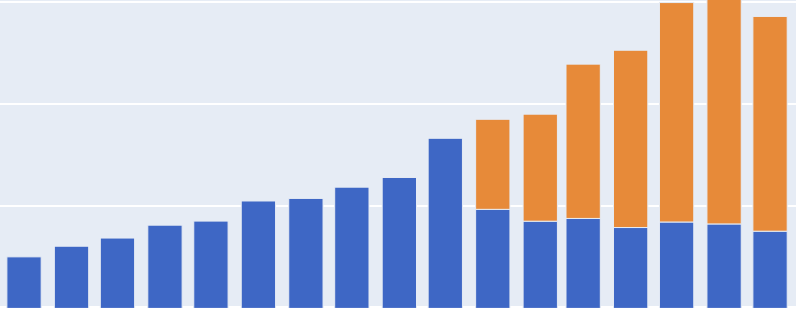
\includegraphics[width=5in]{img/stacked_barchart.png}
  \caption{Stacked bar chart}
  \label{fig2.3}
\end{figure}
\\
\paragraph{Stacked bar chart (Figure 2.2)}
It is particularly suited to analyze the data distribution and focus on the quantity of a certain value with respect to other values. It is the most frequent chart. Different classes of data sharing some common attributes get stacked to render the idea of their quantitative difference.
In this example we see the distribution of two different generations of editors through the years.
\\
\begin{figure}[!ht]
  \centering
  \setlocalecaption{english}{figure}{Figure}
  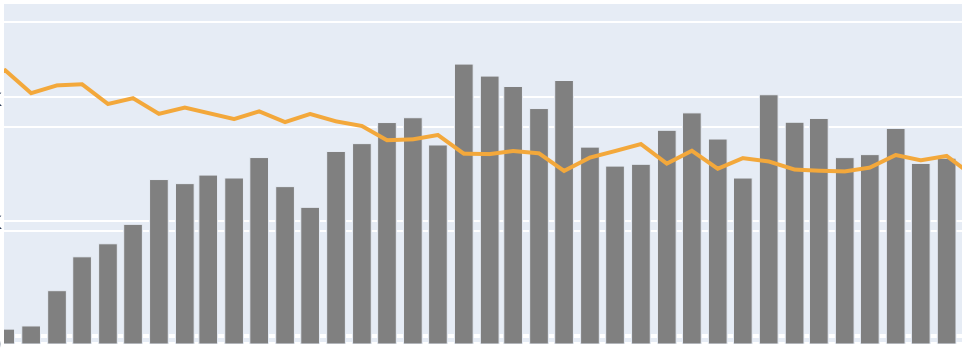
\includegraphics[width=5in]{img/dual_axis_graph.png}
  \caption{Dual-axis graph: line chart and bar chart}
  \label{fig2.4}
\end{figure}
\\
\paragraph{Dual-axis graph (Figure 2.3)}
Helps conveying multiple information at the same time. In fact, in the dashboards it is used in its line chart plus bar chart configuration, thus, it helps the user to analyze the distribution of a certain data class and also compare it to the evolution in time of another class of data. In this example, we can see the distribution of registered editors with respect to the evolution in time of the number of editors that remain active after a certain temporal threshold. Again, this will be explained later.
\pagebreak
\\
\begin{figure}[!h]
  \centering
  \setlocalecaption{english}{figure}{Figure}
  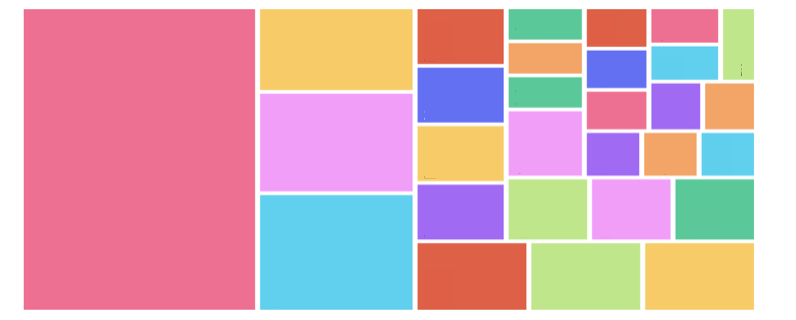
\includegraphics[width=5in]{img/treemap.png}
  \caption{Treemap chart}
  \label{fig2.5}
\end{figure}
\\
\paragraph{Treemap chart (Figure 2.3)}
Finally, the Treemap chart. It is a special graph used to represent the quantitative distribution of certain data classes with respect to all the other data classes considered in the current analysis. \\It is preferred to a pie chart visualization because the comparison between rectangular shapes is clearer than the contrast between circular sectors. Each colorful square can be expanded, to reveal other information about the current object, in this case the current language.\cite{treemap}\\
In the dashboards it is used to visualize the Meta-Wiki participation of the all the Wikipedia language communities.

\section{Dash}
\label{sec:dash}

Dash is the web framework on which the Plotly apps run. It is tailored to create visual dashboards in an extremely simple way. \cite{dash}\\
The entire dashboards layout is built with Dash. There is no HTML, no CSS nor JavaScript.\\
The layout is, however, built with components of the HTML Python module that allows to place HTML classic components, like \verb#div# container or radio buttons, and handling them with a JSON-like syntax. These components directly communicate with the Plotly graphs thanks to the Dash functions, or callbacks, that feed the information coming from them to the Plotly charts, making them interactive. Not only the graphs are interactive, the whole page is: by selecting the desired vital sign, the layout will automatically display the respective dashboard.

\lstset{frame=lines}
\lstset{label={lst:code_direct}}
\lstset{basicstyle=\footnotesize}
\lstset{caption=Structuring the Dash layout}
\begin{lstlisting}
import dash
from dash import Dash, dcc, html, dbc

html.Div(
        html.P('Select Yearly or Monthly Time aggregation'),
        
        html.Br(),
        
        html.Div(
            dcc.Dropdown(
                id='language',
                multi=True,
                value='English (en)',
                style={'width':'490px'}
            ), style={'display':'inline-block','width':'500px'}
        )
    )
    
\end{lstlisting}

From the code snippet above, we can clearly see the absence of any HTML code.
The whole layout is implemented using Python scripts like this.\\
Dash has many libraries as well, such as dash core components (\verb#dcc#) and dash bootstrap components (\verb#dbc#), that provides HTML components with pre-built CSS style, in order to help us build an homogeneous and  elegant web page. Since we want to focus on the dashboards, the layout is designed to be minimal.\\
From the example above, in fact, we can see a drop down in a HTML \verb#Div#. This element comes from the \verb#dbc# library and provides a simple custom drop down menu:
\begin{itemize}
    \item \textbf{id}: since it is an HTML element, we can set its identifier
    \item \textbf{multi}: we can set if it must contains more than one choice
    \item \textbf{value}: it allows us to set the default value, in this case the English language
    \item \textbf{style}: we can add other information about the CSS style
\end{itemize}

All these graphic components hide more than what we see: they are the interface through which we can interact with the Plotly charts.
We can bind these components with functions, called Dash callbacks, that communicate directly with the Graph objects.\\
We also said that Dash is responsible for the whole business logic of the web applications. Let us take a look at the callbacks and how they are defined.

\lstset{frame=lines}
\lstset{label={lst:code_direct}}
\lstset{basicstyle=\footnotesize}
\lstset{caption=Dash callback for URL update}
\begin{lstlisting}
import dash
from urllib.parse import urlparse, parse_qsl, urlencode

@app.callback(Output('page-content', 'children'),
              inputs=[Input('url', 'href')])
def page_load(href):
    if not href:
        return []
    state = parse_state(href)
    return layout1
    
\end{lstlisting}

From the code snippet above we see the definition of a Dash callback.
It works just like a function: we define the input and the output structure, and we write the code to execute. The main thing to notice is that we bind this function to the Dash application with the \verb#@app.callback# string.\\
In this example we are looking at the function that allows the sharing of the visualization with other users: the parameters that are read from the graph callbacks are embedded in the URL, in order to let the page update its HTML components' value with the values read from the URL. In this way, the callbacks will always read the correct parameters. We will read the default ones only if we are visiting the dashboard as a new visitor.\\
In the next chapter, we will have a closer look at this mechanism.\\


\section{Pandas}
\label{sec:pandas}

Pandas is the mediator between front-end and back-end code. \cite{pandas} \\
It is a Python module that is in touch both with Plotly and with the SQL database, managing the data flow between these two components.\\
It is mainly used to encapsulate the result sets coming from the SQL queries asked to the Eurecat Database. Since this data is still too raw, we need to process them in a way that they can work properly with Plotly: we use Pandas objects called Data frames. \\
The Pandas data frames are extremely useful, since they allow us to grab the raw data and envelope them into objects that are much more malleable than their raw form: they have a lot of methods to handle themselves. Let us take a look at how data frames are created:\\

\lstset{frame=lines}
\lstset{label={lst:code_direct}}
\lstset{basicstyle=\footnotesize}
\lstset{caption=Creating a Pandas data frame}
\begin{lstlisting}
import pandas as pd
import sqlite3

conn = sqlite3.connect(database)

SQL_query = '''select * 
            from vital_signs_metrics 
            where topic = 'active_editors' 
                and year_year_month = '''+time_type+'''
                and m1_calculation = 'threshold' 
                and m1_value = '''+user_type+'''  
                and langcode IN (%s) '''%languages

df = pd.read_sql_query(SQL_query, conn)
print(df[:100])
df['percentage']=((df['m2_count']/df['m1_count'])*100).round(2)
    
\end{lstlisting}

First of all, we specify the database with the Sqlite3 connection object \verb#conn#. Then, we create a parameterized SQL query.\\
The parameters of this query are:
\begin{itemize}
    \item \textbf{time type}: it specifies the time aggregation of the final chart, that can be yearly or monthly.
    \item \textbf{user type}: it specifies if we talk about active editors or very active editors.
    \item \textbf{languages}: it determines the desired languages on which we want to do our research.
\end{itemize}
The query is then passed to the database and, at the same time, the result set is put into the data frame \verb#df#. We then print it to ensure that it is the correct desired data set.\\
Finally, we create a new data frame column from already existing ones. In the example above, we create a percentage column.\\ 
If we wanted to do this via SQL, we would have to change the query and thus, we would have put two different things at the same time, violating the Separation of Concern principle \cite{soc}.\\ Instead, with this method we can launch a high level query and then refining it with Pandas. This is much more convenient since we can separate the creation of the raw result set and then the refining phase, making it easier to eventually debug.\\
Later on we will have an in-depth view on how Pandas and Plotly work together.

\section{Architecture}
\label{sec:architecture}
Now that the Python module have been described, this section illustrates how they are structured.

\begin{figure}[!ht]
  \centering
  \setlocalecaption{english}{figure}{Figure}
  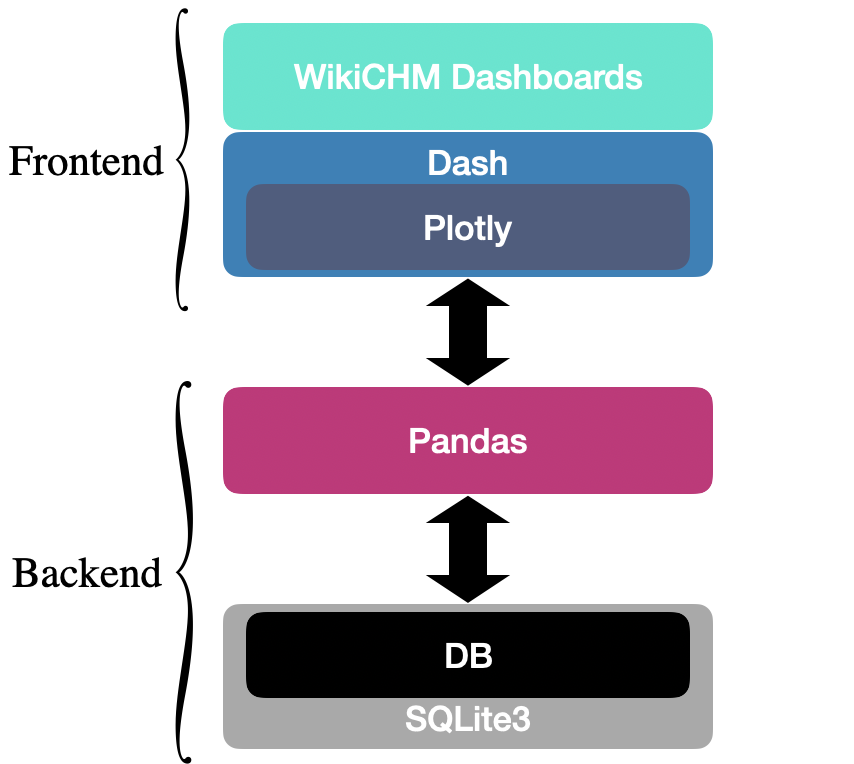
\includegraphics[width=3in]{img/architecture.png}
  \caption{Dashboards architecture}
  \label{fig:arch}
\end{figure}

The Figure \ref{fig:arch} is a high-level definition of the architecture of the visual dashboards. \\
Every level of this structure has been made with ad-hoc Python modules.\\
Let us describe them with a top-down approach:
\begin{itemize}
    \item \textbf{Plotly}: every dashboard's graph is made with the Python library for data visualization. It is contained into Dash web framework to allow the interaction between the user and the HTML components.
    It is what the user actually sees and interacts with
    
    \item \textbf{Dash}: the charts run in a web container, realized with a Python module that allows the creation of web applications. Dash automatically manages every web-related aspects such as the building of the entire layout that can totally change at run-time, creating the website to which the user can access to. \\
    Dash is also responsible for the functions that make the dashboard interactive and for the dynamic layout
    
    \item \textbf{Pandas}: the data plotted are handled with the widely-used data manipulation Python library, handling and managing the exchange of data between the underlying DBMS and the above layers. It is the mediator between the front-end dashboards and the back-end data.
    
    \item \textbf{SQLite3}: this low-level module provides the connection with the relational database, created by the Eurecat researchers, and mainly acts as its DBMS. It is the responsible for raw extraction of the data.
\end{itemize}
Every layer of the structure dialogues with its neighbour.
The data flow bottom up: from the database to the Wiki Community Health Metrics dashboards.\\
Each component captures the output of the underlying layer, elaborates it, and feed its own result to the overlying one.
All these Python modules have been chosen for their mutual compatibility, in particular Python, Dash and Pandas to ensure a smooth and robust workflow.

\space
      \chapter{Implementation}
\label{cha:implementation}

The vital signs Dashboard shows us different graphs with different data visualization about specific aspects of the health status of Wikipedia. Despite their overall similarity, each of them is built differently from the others due to its peculiarity.\\
In this chapter we are going to have an in-depth look at how the code is structured and at the actual implementation of each different dashboard.\\

\section{Business logic}
\label{sec:business_logic}

The main idea behind every charts is the following: we read the input from the HTML components, we process it in some way to make it compliant with the SQL queries, then we capture the outputs and feed them to the Plotly chart.\\
This whole interaction between the Dash layout and the Plotly charts is done with Dash asynchronous functions: the callbacks. Each graph has its callback that is linked to some of the HTML components and each time the user interacts with one of them, the function is called.\\
The same is done for the highlights since they also need information about the current visualization in order to adapt the captions.\\
There is also a higher level of dynamics, regarding the whole layout: in the previous chapter we have looked at an example of a Dash function that changes the layout according to the URL parameter. This whole mechanism can be described as follows:
\pagebreak
\begin{figure}[h]
    \centering
    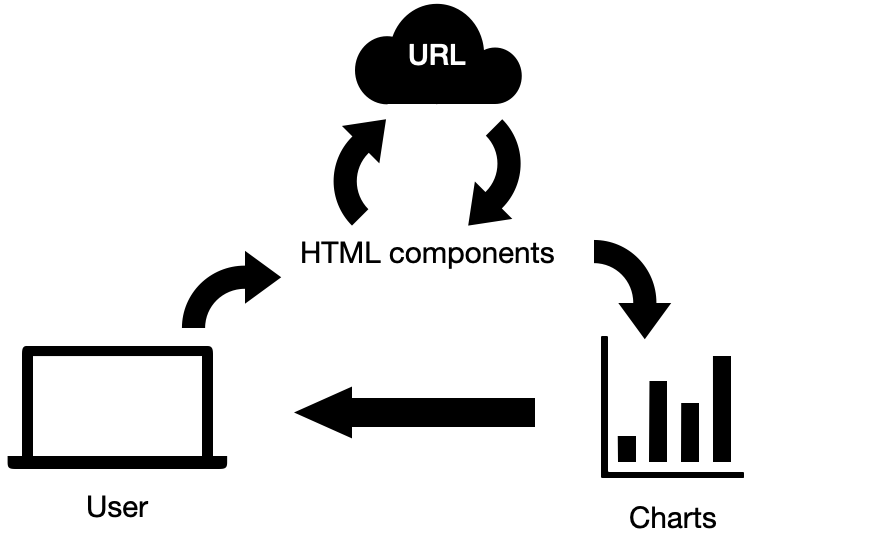
\includegraphics[width=200px]{img/callback-loop.png}
    \setlocalecaption{english}{figure}{Figure}
    \caption{Dash callback loop}
    \label{fig:callback_loop}
\end{figure}
\\
The user interacts with the HTML components, setting some parameters. When they change value, a function is activated that embed each parameter into the URL. As soon as the URL changes, a function parses it, retrieving the parameter and applying the change to the same HTML components that activated the loop. The main goal of this is that by changing the vital sign from the drop down menu, the layout is changed accordingly. Moreover, the respective vital sign callback is called, kick-starting the creation of the dashboard that will return the graph\footnote{For some vital signs there is more than one graph, even with one language only}. \\
In this way, our visualization coordinates are preserved: if we select some parameters for a certain vital sign, like Italian and French on very active editors, these choices will be maintained when we change vital sign, allowing the comparison of the same communities under different health metrics.\\
There is also another effect: by sharing our link of the current page with someone else, they will see exactly our same visualization. We remind that the goal of the project is, in fact, sharing knowledge.
We will now see each callback of the different \textit{Vital signs}.

\section{Editors}
\label{sec:editors}
The first dashboard is about editors: the users that are actively involved in the Wikipedia project by writing and editing the Wikipedia pages.\\
Based on the number of their monthly contributions we can split them into two categories: active editors and very active editors.\\
Active editors are the users that edit at least five times per month, while very active editors are those who edit at least 100 times per month.\\
From the graph in Figure \ref{fig:editors} we see the number of active and very active editors in different language communities. Since we are interested into seeing how these numbers changed over time, a line chart is provided.\\
We are also interested into comparing these values across different languages. In fact, the graph allows the visualization of different contemporary traces representing the evolution of the number of editors in different languages (with different colors).

\begin{figure}[h]
    \centering
    \includegraphics[width=470px]{img/active_editors.png}
    \setlocalecaption{english}{figure}{Figure}
    \caption{Active editors dashboard}
    \label{fig:editors}
\end{figure}

%\includegraphics[scale=0.4]{active_editors.png}

\subsection{Editors implementation}
\label{sec:editors_callback}

The Active editors dashboard is perhaps the simplest one.\\
The graph directly reads which information to display from the interactive components `` ``Language",  ``Editors" and ``Time aggregation".\\
First, the function reads the language into a list. Then, the whole languages names like ``Italian (it), German (de)" are converted through a dictionary, called \verb#language_names# into their respective language codes, to make it compliant with the SQL queries. Furthermore, an additional string is created called \verb#params#. This string is very important because in the final query we will search the languages contained in this parameter. We have obtained our first parameter.\\
We proceed to capture the type of editors the user wants to visualize. This can be done by simply filtering the input number called \verb#user_type#. If it is equal to five, then they are active editors, otherwise they are very active editors. In reality, the input number will be passed to the query untouched, since the HTML component has a numeric value behind the literal label. This is our second parameter.\\
Finally, we want to know if to display a monthly charts or a yearly one, and the process is identical to the one described for the numeric value of the editors.\\
Now, after having collected these three parameters, we can build a parameterized query by having a fixed statement and inserting, in the string, the variables containing the parameters. We then run the query to the database using pandas, yielding a data frame containing the desired information. This object is now passed to the actual plotly charts at creation time.\\

\lstset{frame=lines}
\lstset{label={lst:code_direct}}
\lstset{basicstyle=\footnotesize}
\lstset{caption=Creating a line chart}
\begin{lstlisting}

fig = px.line(
             dataframe=df,
             x='year_month',
             y='m1_count',
             color=df['language_name'],
             height=500,
             width=1200,
             title=incipit+' Users',
             labels={
                     "m1_count": incipit+" Editors ",
                     "year_month": time_text,
                     "language_name": "Projects",
                 },
            )
    
\end{lstlisting}

From the example above we can see the code responsible for the creation of a line chart. It is done using plotly express, the sub-module of plotly.\\
We can also see how we specify the data source, the data frame, and which data column we want to put on the x-axis and on the y-axis.\\
We can also see some other keywords that are useful to improve the visualization of the graph: we can set a title to enhance its readability, we can specify its size and we can also create a map that provides more readable labels for the data columns.\\
Finally the dashboard is ready to be deployed.

\section{Retention}
\label{sec:retention}

The first vital sign is Retention and it measures the percentage of new editors that survives 60 days\footnote{Retention period is not fixed but can be chosen from different time periods: 24 hours, 30, 60, 365 and 730 days} after the first edit. Survivors are meant as those users which keep editing after the time threshold. We are interested in the capability of a certain community of keeping its editors engaged, in order to understand if and why editors are leaving Wikipedia.\\
In this dashboard we can see the retention rate of one or more language communities, along the timely distribution of the registered users. From Figure \ref{fig:retention}, we can see that the graph is actually a dual-axis chart: on the left y-axis, as bars, we have the number of registered editors, while on the right y-axis we have the retention rate displayed as an orange line.

\begin{figure}[h]
    \centering
    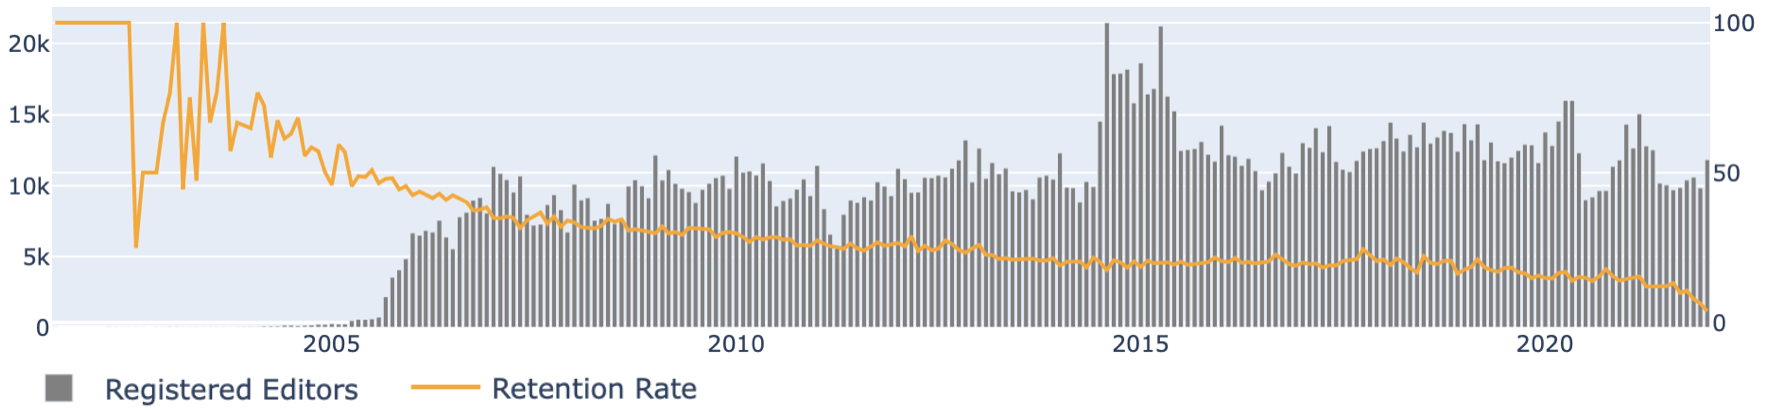
\includegraphics[height=140px, width=480px]{img/retention.png}
    \setlocalecaption{english}{figure}{Figure}
    \caption{Retention dashboard}
    \label{fig:retention}
\end{figure}

\subsection{Retention implementation}
\label{sec:retention_callback}

The retention dashboard is quite different from the previous dashboard and from the following ones since it is not a normal chart, but a dual chart.  Due to the high-level nature of plotly express, this module was not useful to code a dual-axis chart. Thus, the graph objects module was used; in particular the \verb#make_submodule()# method.

\lstset{frame=lines}
\lstset{label={lst:code_direct}}
\lstset{basicstyle=\footnotesize}
\lstset{caption=Creating a dual axis: line chart and bar chart}
\begin{lstlisting}

fig = make_subplots(
    specs=[[{"secondary_y": True}]])

fig.add_bar(
    x=df1['year_month'],
    y=df1['m1_count'],
    name="Registered Editors",
    marker_color='gray')

fig.add_trace(
    go.Scatter(
        x=df2['year_month'],
        y=df2['retention'],
        name="Retention Rate",
        hovertemplate='%{y:.2f}%',
        marker_color='orange'),
        secondary_y=True)
    
\end{lstlisting}

Here we can see the code responsible for the realization of the Retention dual axis. \\
First we create a figure with a secondary vertical axis. Then, we set which type of charts will populate this figure: we add a bar chart, for registered editors, and a line chart, for the retention rate, with \verb#go#. To enhance the readability of the latter, we use the keyword \verb#hovertemplate# to show the retention values when the cursor passes over the line.\\
We remind that our goal is to visualize Wikipedia communities health values and to compare them. In fact, when we select multiple languages in the drop down menu, one Retention graph for each language will appear. This feature is similar to the one of the following graph, but from the back-end prospective it is fundamentally different.\\
We will later discuss the use of a fundamental keyword, \verb#facet_row#, but for our current understanding we can limit to the fact that the mechanism of the Retention graphs is unlike the others.\\
To duplicate the Retention graphs based on the number of input languages, a for loop has been applied: when we dynamically return the layout, we also call the function related to that vital sign and, in this case, we return more than one retention graph, each one with a different language from the input.

\lstset{frame=lines}
\lstset{label={lst:code_direct}}
\lstset{basicstyle=\footnotesize}
\lstset{caption=For-loop to return multiple charts}
\begin{lstlisting}
array=[]
res = html.Div(children=array)

for x in language:
    fig=retention_graph(x, retention_rate, len(params))
    array.append(fig)

return res
\end{lstlisting}

In this way we by-pass the problem of \verb#go# not supporting the \verb#facet_row# keyword. We simply create multiple graphs and we return it all, yielding the visualization in Figure \ref{fig:multiple_retention}.

\begin{figure}[h!]
    \centering
    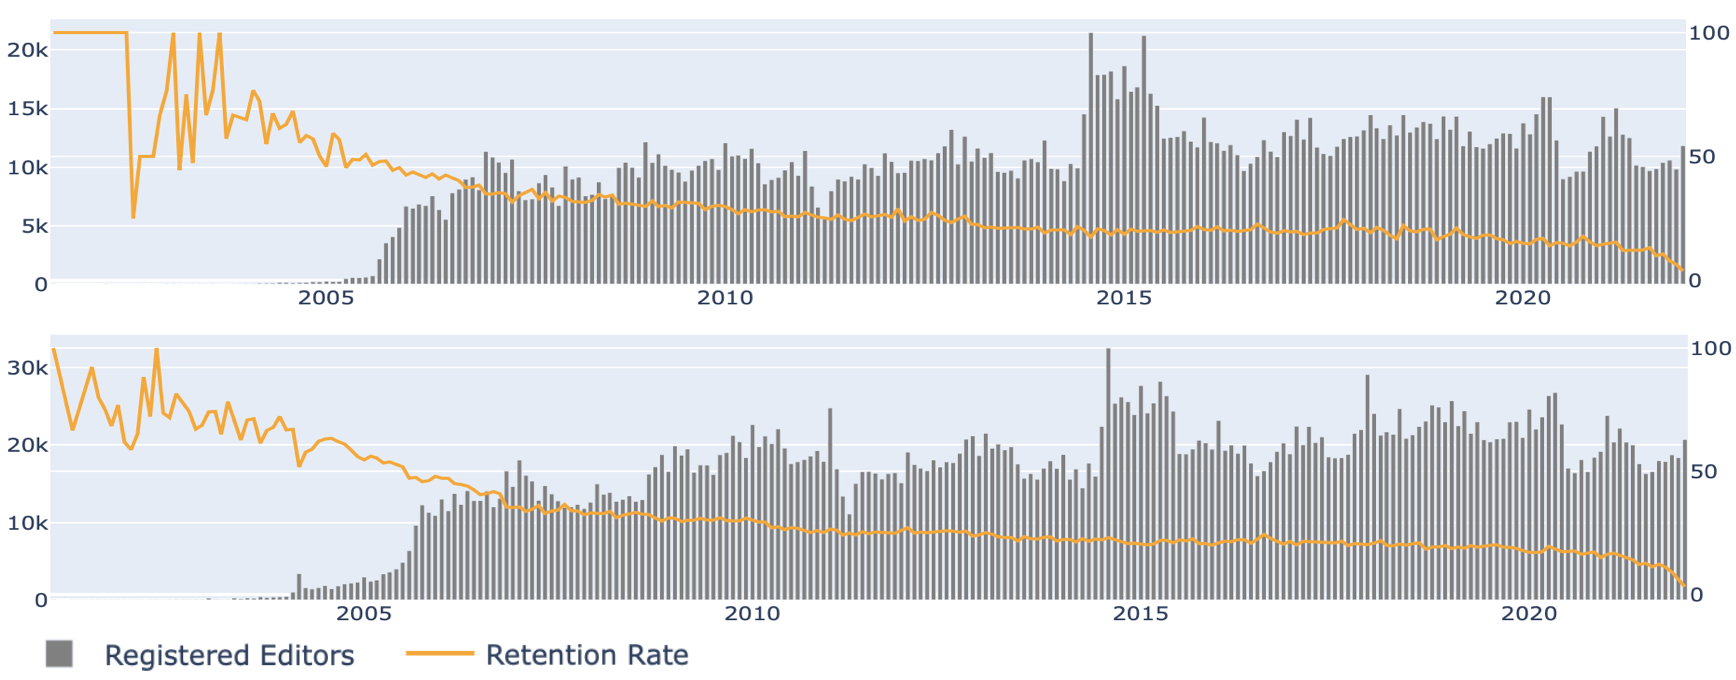
\includegraphics[width=470px]{img/multiple_retention.png}
    \setlocalecaption{english}{figure}{Figure}
    \caption{Multiple retention rates}
    \label{fig:multiple_retention}
\end{figure}

In Figure \ref{fig:multiple_retention} we can see an example of the retention graphs when multiple language are selected, in this case Italian and German.\\
This method has some drawbacks though: mainly, the visualization is not as compact as it would be with the \verb#facet_row# method, in fact the titles and the legends are repeated.

\section{Stability}
\label{sec:stability}

The second vital sign is Stability and it measures persistence of active and very active editors, as well as by the succession of the various generations of editors over time. It is a useful indicator since we want to know if a certain language community is able to attract new editors, called "fresh", and at the same time if it has solid community composed by long-term engaged editors.\\
For this metric it is convenient to classify the editors based on the number of months for which they kept editing Wikipedia's pages. We have different bin from one month to more than 24 months. The editors that keep editing for one month in a row are defined as ``fresh editors".\\
In the stacked bar chart below we can see that each bin of continuous activity is colored differently.

\begin{figure}[h]
    \centering
    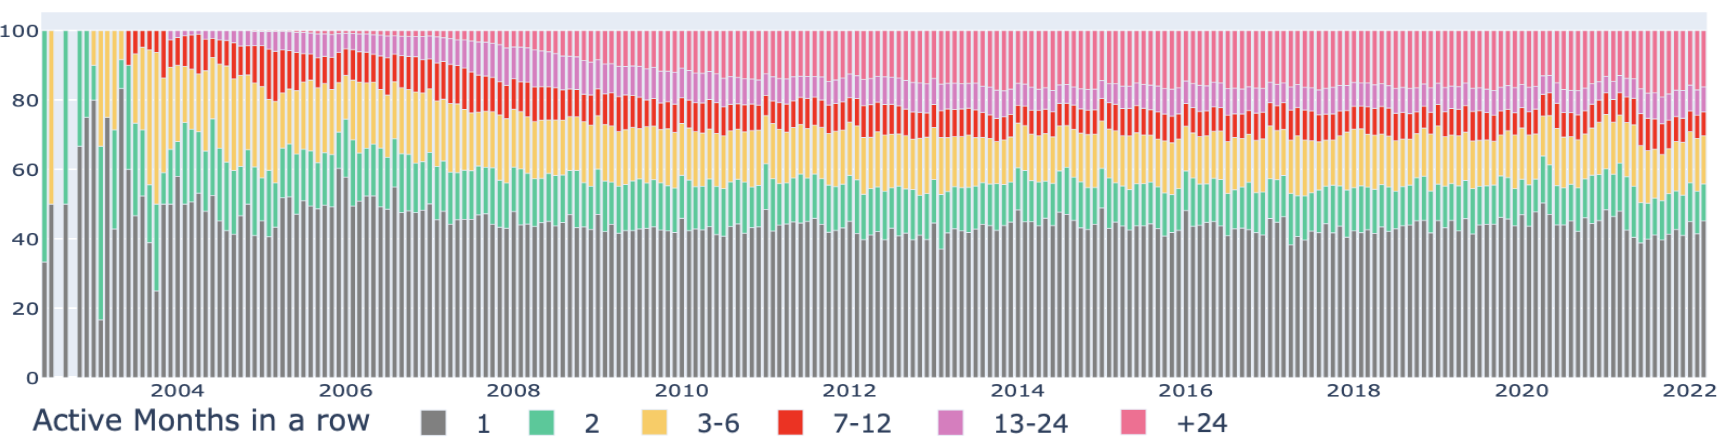
\includegraphics[width=460px]{img/stability.png}
    \setlocalecaption{english}{figure}{Figure}
    \caption{Stability dashboard}
    \label{fig:stability}
\end{figure}

The persistence of each class of editors is represented in percentage, but it could be shown by absolute values as well, through the radio buttons of the HTML components.\\

\subsection{Stability implementation}
\label{sec:stability_callback}
The stability metric is the one that introduces the most common graph in the dashboards: the stacked bar chart.\\
Despite it being different from the line chart, this type of visualization has been realized in a very similar way. First, we query the data from the database, reading the input parameter for the languages, the type of editors that can be active or very active, and the type of value that we want to see, percentage or absolute. This parameter, called \verb#value_type#, will not be included in the query, but it is necessary for the correct visualization of the chart: if the user wants to have the absolute values, nothing happens; on the other hand, for a percentage view we have to create a new data column by dividing the number of a given class of editors by the total number of editors in that month.\\
After having retrieved the data, we create the final plot using the Plotly Express \verb#px.bar()# method.

\lstset{frame=lines}
\lstset{label={lst:code_direct}}
\lstset{basicstyle=\footnotesize}
\lstset{caption=Creating a stacked bar chart}
\begin{lstlisting}
fig = px.bar(df,
             x='year_month',
             y=value_type,
             color='m2_value',
             text=value_type,
             facet_row=df['language_name'],
             width=1200,
             height=height_value,
             color_discrete_map={"1": "gray",
                                 "2": "#00CC96",
                                 "3-6": "#FECB52",
                                 "7-12": "red",
                                 "13-24": "#E377C2",
                                 "24+": "#636EFA"},
             labels={"year_month": time_text,
                     "m2_value": "Active Months in a row",
                     "m2_count":  incipit+" Editors"})
\end{lstlisting}
 %the color map and facet_row
We can observe two important keywords: \verb#color_discrete_map# and \verb#facet_row#.
With the first one we set a dictionary that maps our data column to specific colors, in order to have the full control on the final visualization. In this example it is important to avoid using similar colors in order to ensure the contrast between each editor class.
The mapping can be seen in the legend on the right in Figure \ref{fig:stability}.
The second keyword, \verb#facet_row#, is essential for the dashboards. We previously talked about this keyword in retention, explaining how we mimed its mechanism with a for-loop. \\
The \verb#facet_row# attribute \footnote{ facet row is an attribute specific of Plotly express} allows us to set a data column from the data frame, in order to multiply the graph based on each different value of that column. In this example and in the majority of the dashboards we use the \verb#langcode# data column. In this way, we will have a different visualization for each input language, allowing the comparison of the vital signs across the language communities. A meaningful milestone for the WikiCHM project.\\
\\
In Figure \ref{fig:multiple_stability} below, we can observe the result of the
so called ``faceted graph" that yields a more compact view than the for-loop method: for example, there is only one legend for all the charts and each of them is identified by the language on the right.\\
We can also observe that the size of the two graphs is smaller compared to the previous Figure \ref{fig:stability}. This is due to the fact that having many languages, thus many different graphs at their maximum size, would rapidly crowd the page in a way that would prevent making comparison between the languages at the top and the ones at the bottom. We in fact decided to dynamically reduce the size of the graphs, preventing them from becoming too small to be analyzed. However, a maximum of five languages at a time is recommended.

\begin{figure}[!h]
    \centering
    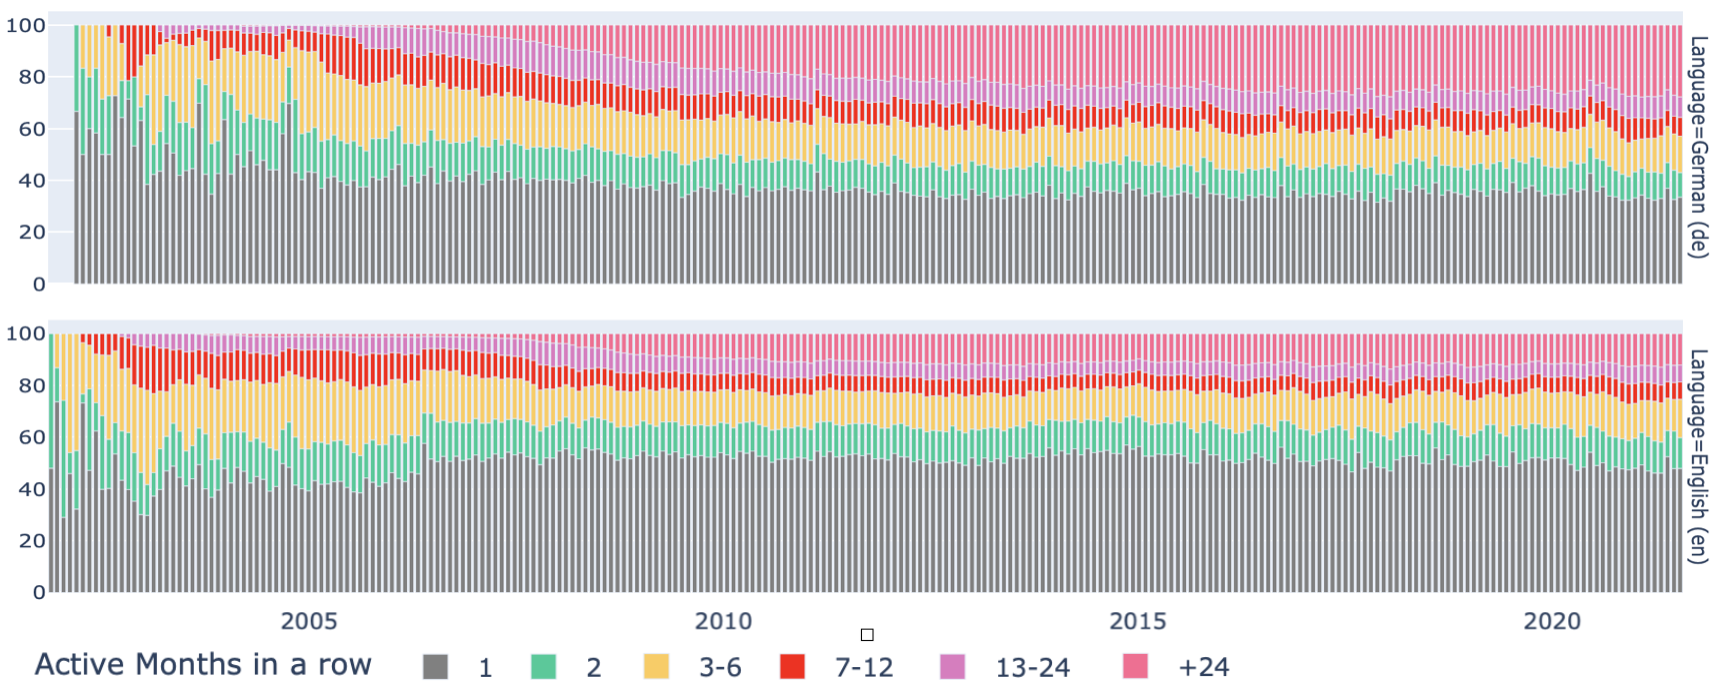
\includegraphics[width=470px]{img/multiple_stability.png}
    \setlocalecaption{english}{figure}{Figure}
    \caption{Faceted stability}
    \label{fig:multiple_stability}
\end{figure}

\section{Balance}
\label{sec:balance}

The third vital sign is community Balance. It measures the ability of a certain community of maintaining an equal proportion of old and new contributors. Previously, in stability, we monitored the distribution of some community's editors. This time, we measure the interaction of the community towards the editors, in particular how well a certain language manage the phenomenon known as ``generational change". For a better understanding of this metric, it is useful to define the concept of "generation of editors": a generation is considered to be five years. This time we discriminate the editors based on their temporal belonging, not on their continuous contribution.\\
In this visualization we can see different colors representing the different generations, from the birth of Wikipedia until our current days (and beyond).
The stacked bar chart is very convenient: for a given year, or month, we can observe the actual distribution of different generation of user, enabling the possibility of doing quantitative analysis. As was said before, the metrics support absolute and percentage values. In this case, a percentage visualization is recommended.

\begin{figure}[h]
    \centering
    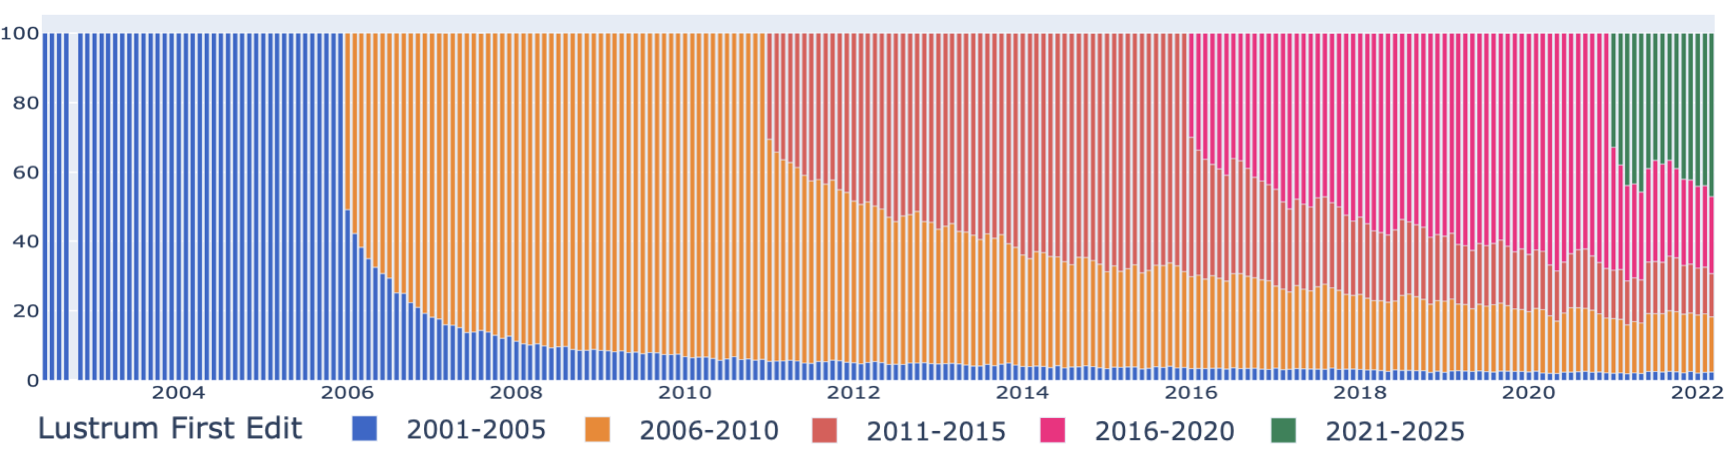
\includegraphics[width=470px]{img/balance.png}
    \setlocalecaption{english}{figure}{Figure}
    \caption{Balance dashboard}
    \label{fig:balance}
\end{figure}

\subsection{Balance implementation}
\label{sec:balance_callback}

The function related to the Balance metric is very similar to the stability one. Thanks to this similarity we take the opportunity to discuss again the basic workflow of each callback.\\
The Dash function, linked to the Dash app, takes as inputs some components' value of the web app layout. In this case, we consider the selected languages, active or very active editors, absolute or percentage values and the timely aggregation of the chart, that can be yearly or monthly; usually, a yearly chart produces more general and meaningful representation of the data and its trends, while a monthly time aggregation favours a discrete and finer-grain data analysis.\\
Then, after having processed the input in order to make them SQL-compliant, we feed them to a parameterized query, that will produce a result set later captured in a Pandas data frame, convenient for the Plotly charts.\\
Finally, we create the figure, in this case a stacked bar chart, that is coded exactly as a common bar chart. We first set the core attributes, like which data column must be placed on the x-axis, y-axis and the \verb#facet_row#, and then the style attributes, like the title, the labels and the size.Once everything is ready, we return the figure to the function responsible for the dynamic layout, displaying it in the appropriate HTML \verb#div#.

\section{Special functions}
\label{sec:special_functions}

The fourth vital sign is called Special functions. It is about editors which hold a certain role that allows them to perform special actions in Wikipedia. In particular, we have two distinct roles: Technical functions and Community coordination functions.\\
Since we have two different classes of functions, we have two different graphs. Two different bar charts that, as the previous vital sign, discriminate the editors based on their generation. The colors are in fact the same.\\
It is evident how the two visualizations look very similar, except for the data distribution. In the dashboards they are paired with a descriptive title.\\

\begin{figure}[h]
    \centering
    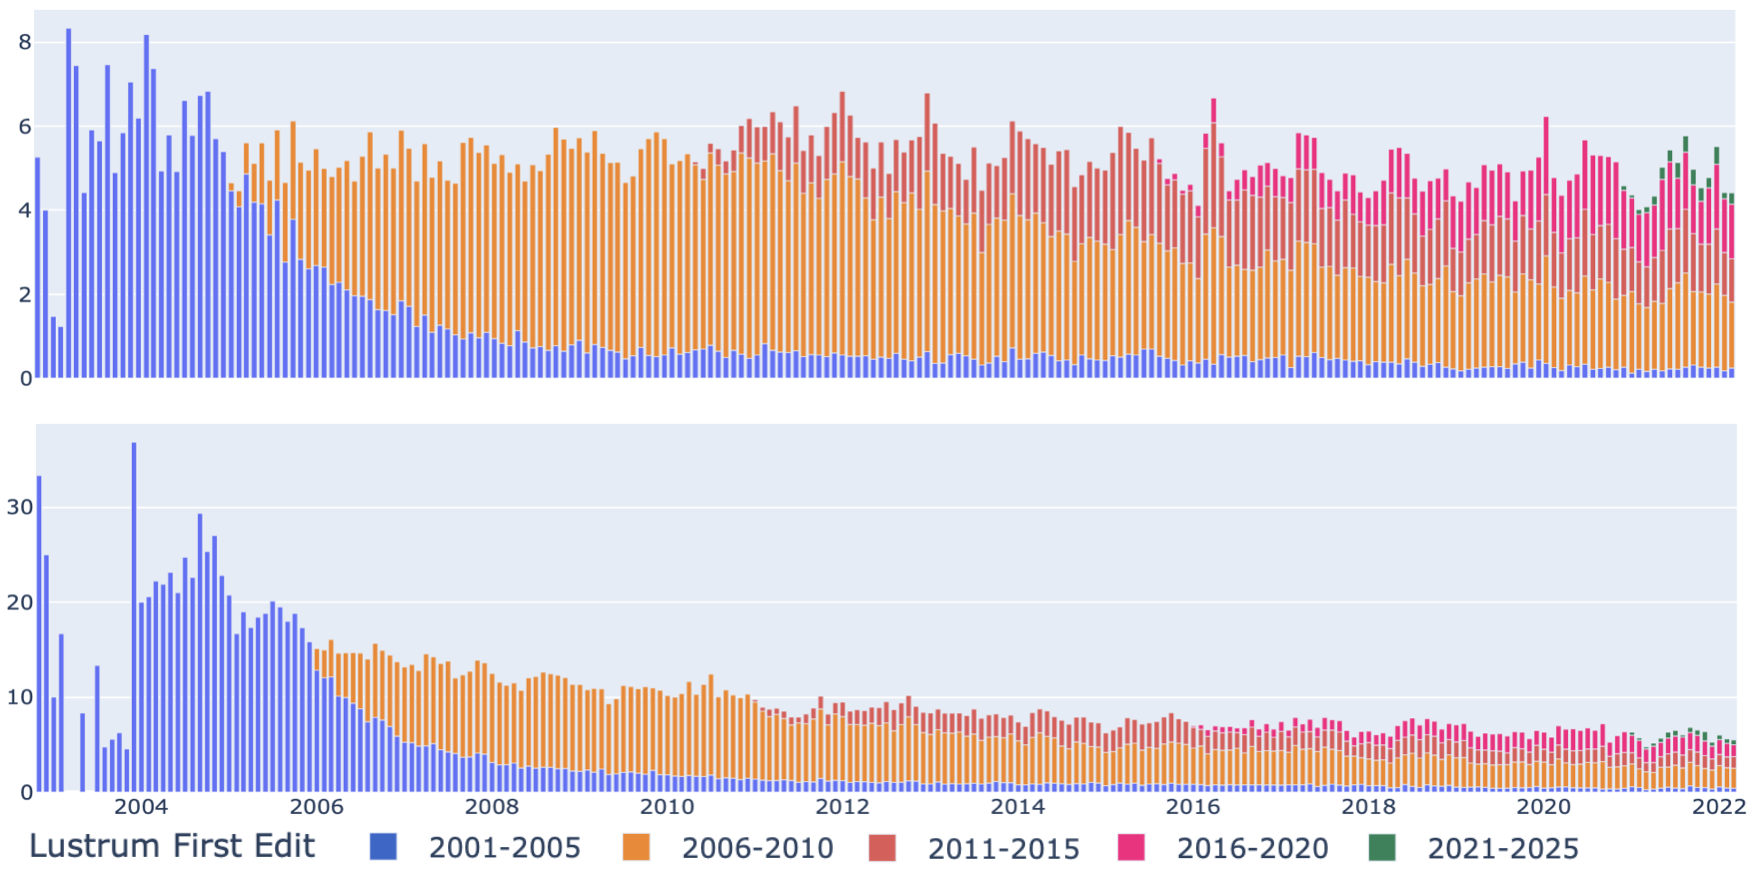
\includegraphics[width=470px]{img/technical_coordinator.png}
    \setlocalecaption{english}{figure}{Figure}
    \caption{Technical and Coordination functions dashboards}
    \label{fig:special_functions}
\end{figure}


\subsection{Special functions implementation}
\label{sec:special_functions_callback}

These two different dashboards have two different callbacks. The two functions work exactly like the other, reading inputs, making a query and creating a figure. To be noted the mechanism with which we return two different graphs in the same layout.\\
We said that the Dash layout contains many HTML components, like the \verb#div# container. There are two of them because some health metric, like Special functions, have two charts to be displayed. In this way we consider this necessity. The functions will output in their respective containers. Also the faceted graph will appear in their intended place.

\section{Admin flags}
\label{sec:admin_flags}

The fifth vital sign is about another kind of specific Wikipedia aspects. This time it is about Administrators. This metric analyzes the distribution in time of editors which hold a position of Wikipedia administrator, with respect to their generation\footnote{The concept of generation is the same for Balance and Specialists}.\\
For this metric the dashboards display three different bar charts.\\
The first one represent the absolute distribution of a certain admin flag over the years. The flag is chosen through the HTML interactive interface.\\
Looking at the charts in Figure \ref{fig:admin} we move to the right to find the second graph: it is a compact view of the first one, since it sums up the editors number discriminating on their generation. The same color as the previous metrics has been kept to enhance the readability and preserve continuity.\\
At the bottom of the Figure \ref{fig:admin}, the third graph is found. It is about the percentage distribution of the previously mentioned admin flag. The title of the graphs changes as the chosen admin flag changes.\\
This time we do not divide the editors in different classes, because we are interested only in the percentage distribution.\\

\begin{figure}[h]
    \centering
    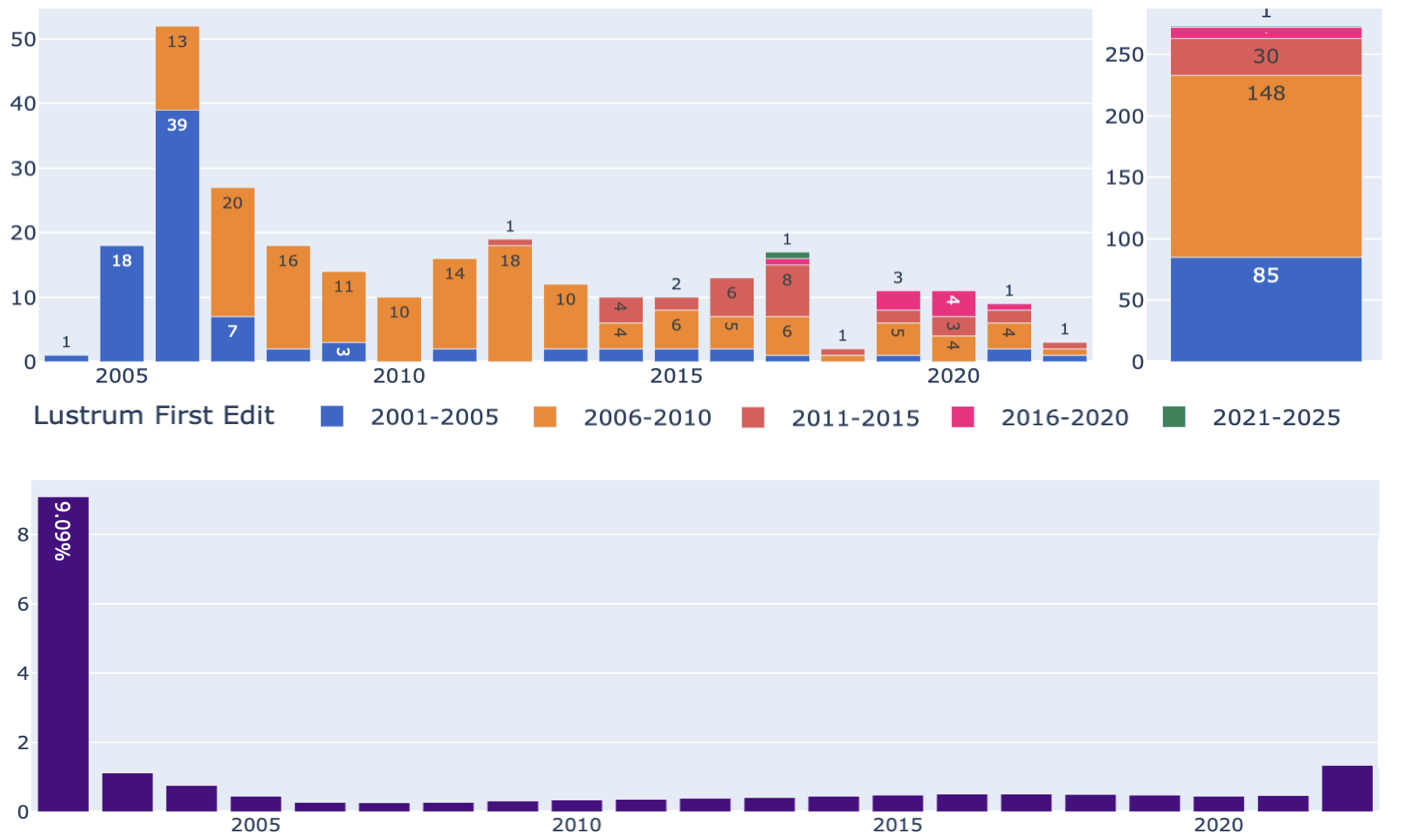
\includegraphics[width=470px]{img/admin.png}
    \setlocalecaption{english}{figure}{Figure}
    \caption{Admin flags dashboards}
    \label{fig:admin}
\end{figure}

\subsection{Admin flags implementation}
\label{sec:admin_flags_callback}

The admin flags' callback has an interesting aspect regarding on which data column we decide to \verb#GROUP BY#. We will not explain how the stacked bar chart are created to avoid time-consuming repetition.\\
We focus on the small chart on the right. It may seem like an extension of the first chart and thus bound to it. But in reality, it is an independent figure.\\
The figure itself is created aside, but its data frame is related to the one used by the first graph.\\ 
For the latter, we retrieve the data about admin editors and we group by the time and by the generation, in order to have the data about different temporal belonging on the same column of the x-axis. Instead, for the second graph we group only by generation, to which we refer as \verb#m2_value# in the python script.
Furthermore, since we are only interested in one-dimension of our data, the absolute values, a new empty data column is created and it is used as the x-axis of this figure, yielding a compact view of our data.
%image? who knows

\section{Global community}
\label{sec:global_community}

The sixth and last vital sign brings the attention to the Global community of Wikipedia. \\
Since Wikipedia is a community project, the participation of each local community to the global one is essential for making their voices heard and learning from others. In this metric we analyze the linguistic origin of the contributions to a certain language community and the contribution of each Wikipedia language community to the global project.\\
This last dashboard has two different charts to satisfy our two different analysis.\\
The first bar chart visualization display the percentage or absolute distribution of all the contributions coming from every available language, towards the chosen language community.\\
For the second analysis we use a peculiar type of graph: a tree-map. As said before, it sums up the individual contribution of each different language community to the global one. Every language is represented as a colorful rectangle whose dimension is proportional to the percentage value of that language contribution to the Meta-Wiki project \cite{meta}. The rectangles also show some additional details like the percentage value and the absolute value. By clicking on one of them there is a little nice animation that expands the whole rectangle, allowing to analyze the small communities too.

\begin{figure}[h]
    \centering
   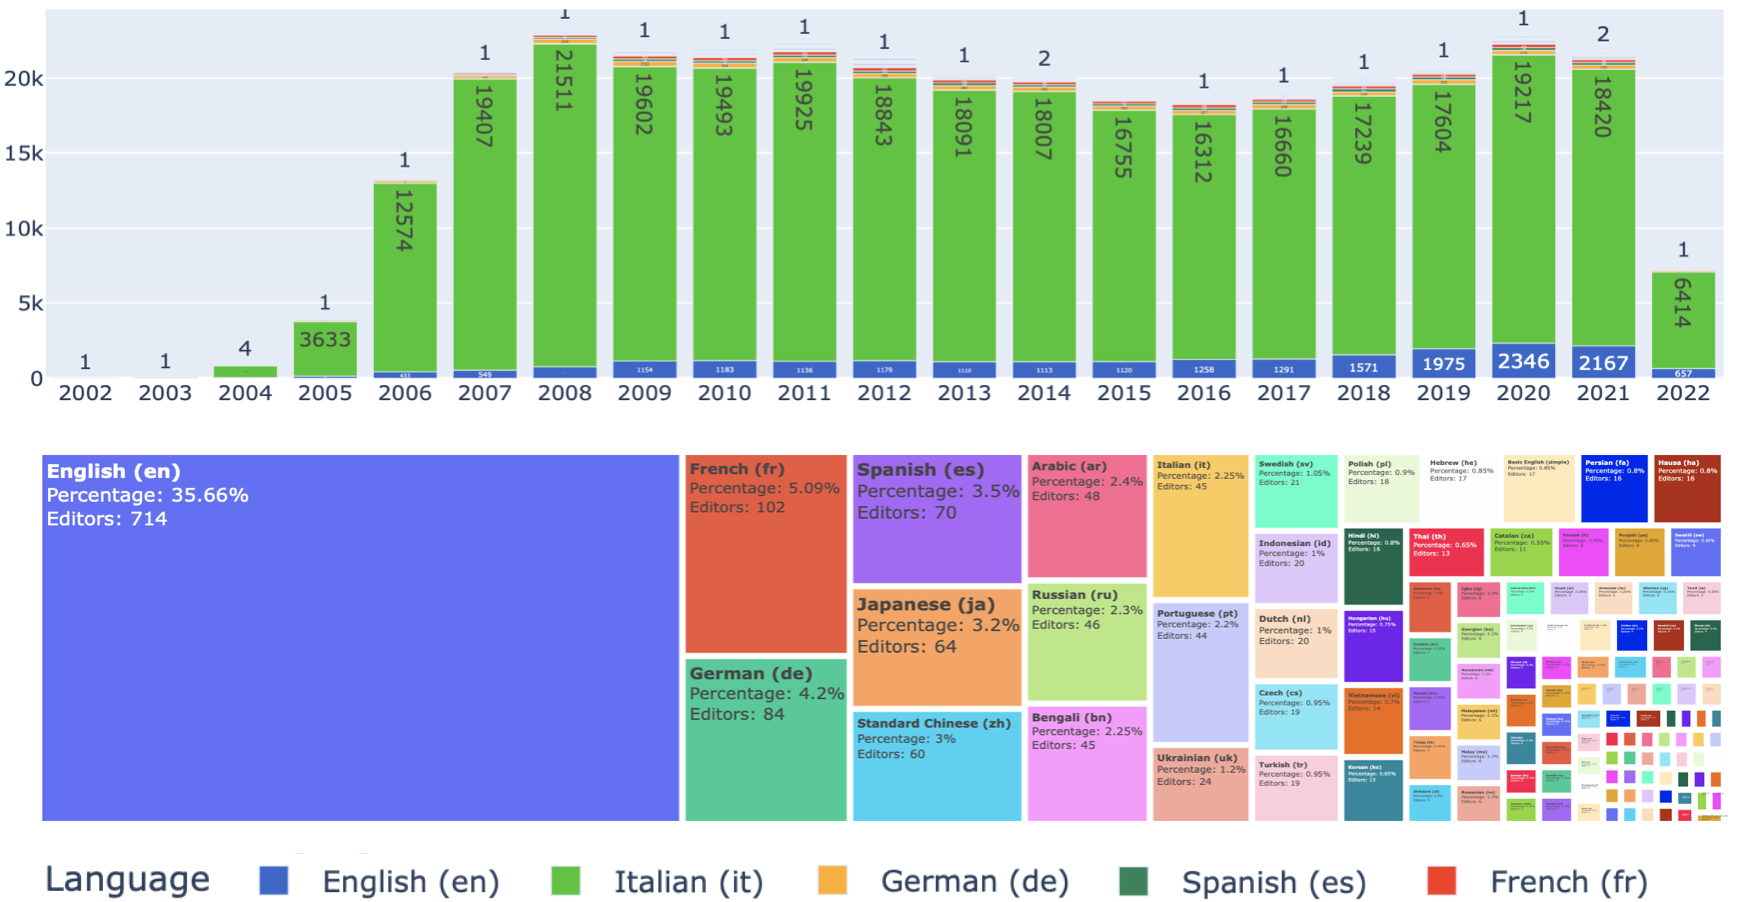
\includegraphics[width=470px]{img/global.png}
    \setlocalecaption{english}{figure}{Figure}
    \caption{Global community participation dashboard}
    \label{fig:global}
\end{figure}


\subsection{Global community implementation}
\label{sec:global_community_callback}

These last dashboards are essential for the project goal since without them we would not have a full picture on the health status of the different communities in Wikipedia. These charts have been realized with a similar code to the others, but this time the colors play an important role since we cannot distinguish different languages in the charts, if not with colors. Unfortunately, there has not been found a way to describe a mapping for every possible language to a unique color since there are simply too many of them. Nonetheless, the results have been considered clearer than what was expected, in particular on the first graph.\\
About the second chart, the tree-map, we used the Plotly sub-module \verb#go#, in a similar way to what was done for the retention visualization. It has been preferred to Plotly Express for its low-level control on the graph figure itself, at the price of a slightly more complex syntax. 
\pagebreak
\lstset{frame=lines}
\lstset{label={lst:code_direct}}
\lstset{basicstyle=\footnotesize}
\lstset{caption=Creating a treemap chart}
\begin{lstlisting}
fig2 = go.Figure()

fig2.add_trace(go.Treemap(
    parents = df2["langcode"],
    labels = df2['language_name'],
    values = df2['m2_count'],
    customdata = df2['perc'],
    text=df2['m2_value'],
    texttemplate = '''<b>%{label} </b><br>Percentage: 
                        %{customdata}%<br>Editors: %{value}<br>''',
    hovertemplate='''<b>%{label} </b><br>Percentage: 
                        %{customdata}%<br>Editors: %{value}<br>
                        %{text}<br><extra></extra>'''))
\end{lstlisting}

A \verb#go.Figure# is created and then we added the tree-map trace, by specifying the common parent for every node (the rectangles) that is the Meta-Wiki topic. Then we set the data column to be textually displayed with the keyword \verb#texttemplate# and to be displayed when we pass over with the mouse pointer with \verb#hovertemplate#. In this way we obtain the visualization in Figure \ref{fig:global} that correctly show us the quantitative distribution of each language communities' contributions to the Meta-Wiki. 

\section{Highlights}
\label{sec:highlights}

In the earlier chapter it was said that the health metrics visualization were paired with automated descriptive labels. In this section we are going to discuss their code and their role. The choice of not talking about them in every single graph was taken due to the fact that the mechanism is the same for every highlight, so we dedicate an entire section to this topic.\\
\\
To enhance graphs' readability we use the Highlights: automated descriptive labels that help us reading the graph and its highest or lowest values. In general, they briefly contextualize the graph and describe what we are looking at.\\
These automatic caption have been coded in a very similar way to the one we used to create the charts: we generate a Pandas data frame with the same technique described before, then we use its data column values to extract the values that will be embedded in some prepared textual statement.
A peculiarity of this mechanism is that the values needed some sort of pre-processing phase: the values had to be casted into a string to be concatenated in the textual statements or the date had to be converted in a user-friendly style like the common ``Month Year" format.\\
\\
In the end, we have at least one function for each graph about the highlights. But to actually place it in the layout we have a dash callback that reads which vital sign has been selected and return the result of the respective highlights function, preserving the dynamicity of the entire layout. In this way, we also ensure the highlights to be up to date with the data selected with the HTML components like the language selected or the time aggregation.


      %\chapter{Results}
\label{cha:results}

In this chapter are reported the results and the trends emerged from the created dashboards. It is shown how intuitive the comparison between different language is. For this purpose it is used a language sample taken from the major European languages, namely Italian, German, French and Spanish. They will be compared under the same vital sign to understand the explanatory power of these interactive visualizations and their potential role in the future steps of the Wiki Community Health Metrics project.
We remind that these measurements can be observed by everyone with the online dashboards\cite{vitalsign}, in order to study different languages from the one reported in this chapter. 

\section{Editors}
\label{sec:editors_conclusion}

We begin with Active editors. We remind they are the editors who edit Wikipedia pages at least five times per month. They are the majority of the editors, reaching up to 88\% of the total editors (considering the major language community). The dashboards show how the number of active editors evolved since the birth of Wikipedia until present days.

\begin{figure}[h]
    \centering
    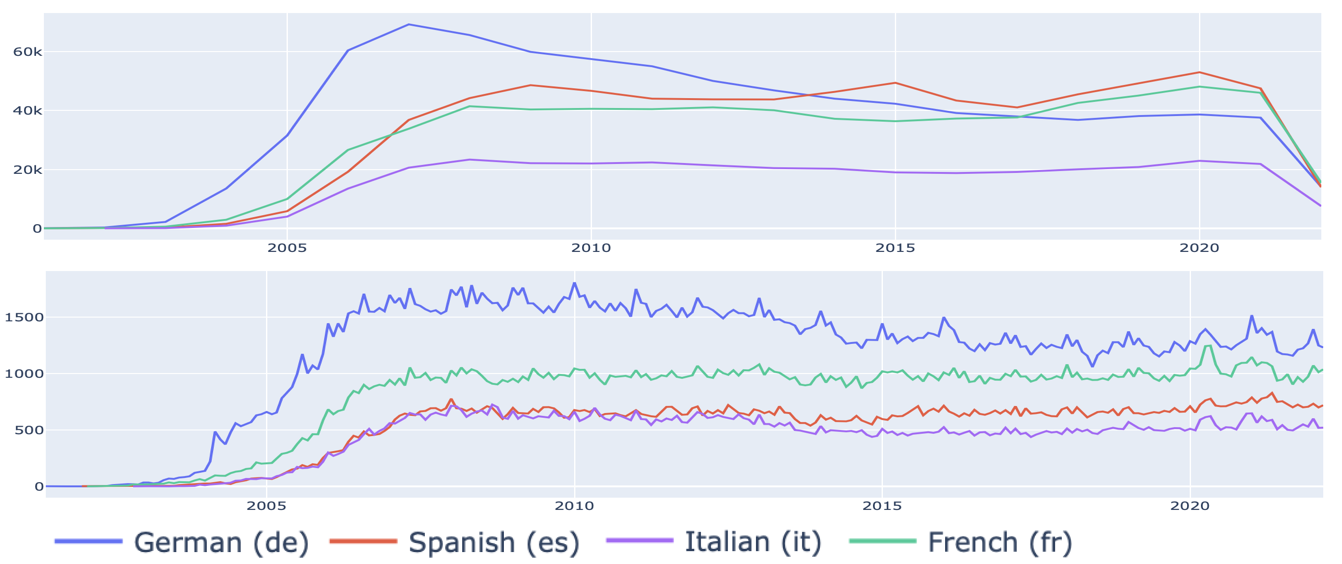
\includegraphics[width=470px]{img/editors_trend.png}
    \setlocalecaption{english}{figure}{Figure}
    \caption{Trend of the major European languages' active and very active editors}
    \label{fig:editors_trend}
\end{figure}

Considering a yearly visualization the first graph in Figure  \ref{fig:editors_trend} shows a general pattern for the major European language communities: after a rapid spike in the early days of Wikipedia, the number of active editors declined until, around the year 2014, they generally reached a stable value.\\
Considering the very active editors and monthly visualization, we get richer charts. The trend in Figure \ref{fig:editors_trend} stays the same but we can also see the number of very active editors fluctuating even during the years themselves: at the beginning of the new year the editors are more than the rest of the year.

\section{Retention}
\label{sec:retention_conclusion}

We now consider the retention dashboards considering the same language sample as before. We remind that the retention rate of a certain community is calculated as the percentage of new editors that survives after a certain threshold from their first edit. We consider the threshold value of 60 days.\\

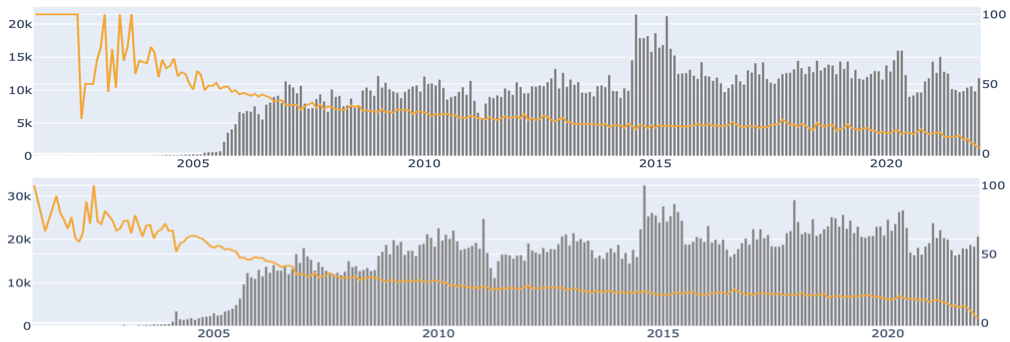
\includegraphics[width=470px]{img/retention_trend.png}
\pagebreak
\begin{figure}[h]
    \centering
    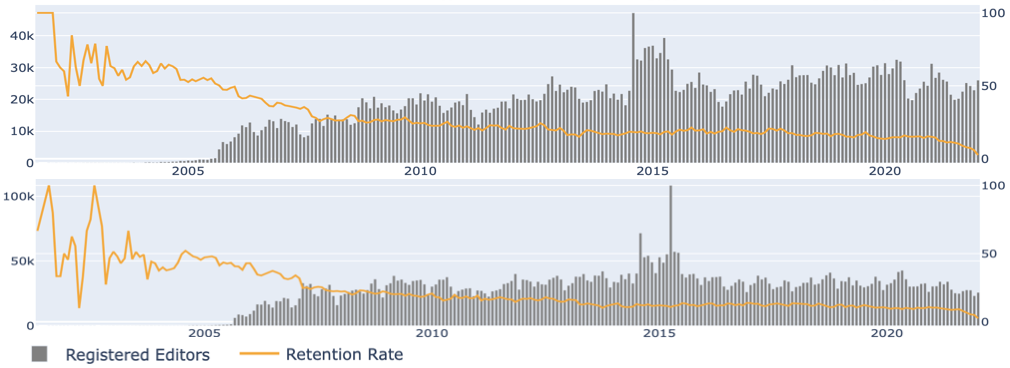
\includegraphics[width=470px]{img/retention_trend1.png}
    \setlocalecaption{english}{figure}{Figure}
    \caption{Trend of the major European languages' retention rates}
    \label{fig:retention_trend}
\end{figure}
\\
From top to bottom: Italian, German, French and Spanish.\\
The retention rates of our language sample show a dramatic declining trend. In every language we observe a common pattern: in the early days we can see a lot of instability, then around the year 2004 the retention rate steadily decreases, especially in the last years. Ideally, the various community should adopt behaviour to revert this trend.


\section{Stability}
\label{sec:stability_conclusion}

Before analyzing the stability trends we remind that the stability of the community is given by the persistence of active and very active editors, as well as by the succession of the various generations of editors over time.\\

\begin{figure}[h]
    \centering
    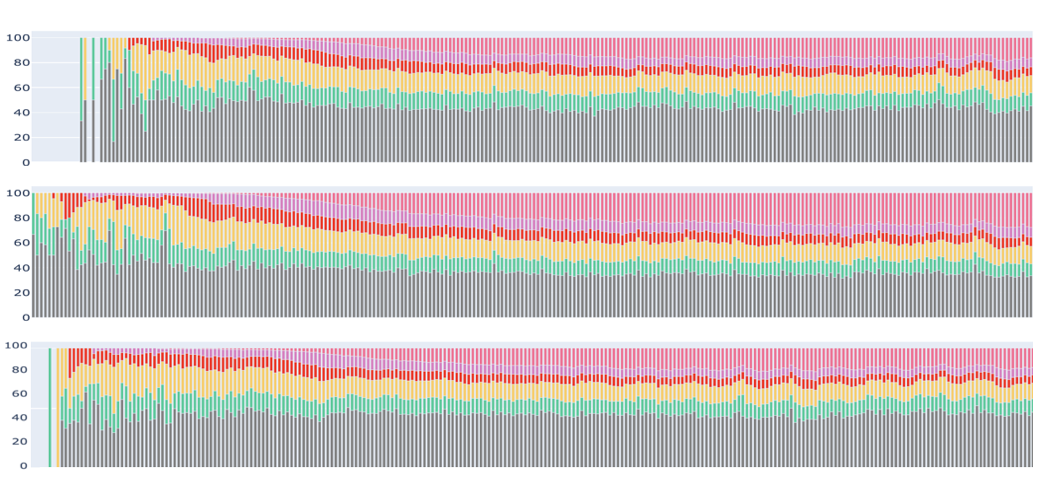
\includegraphics[width=460px]{img/stability_trend.png}
    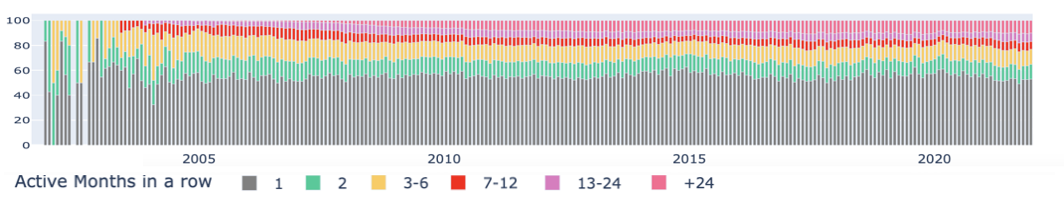
\includegraphics[width=460px]{img/stability_trend1.png}
    \setlocalecaption{english}{figure}{Figure}
    \caption{Trend of the major European languages' stability among active editors}
    \label{fig:stability_trend}
\end{figure}
\pagebreak

As seen in Figure \ref{fig:retention_trend} we have, from top to bottom, Italian, German, French and Spanish stability values.\\
Among active editors, the greater percentage of editors keeps editing for one month. Thus we could deduce that active editors tend to be volatile and less persistent. This trend is consistent across the whole language sample.\\

\begin{figure}[h]
    \centering
    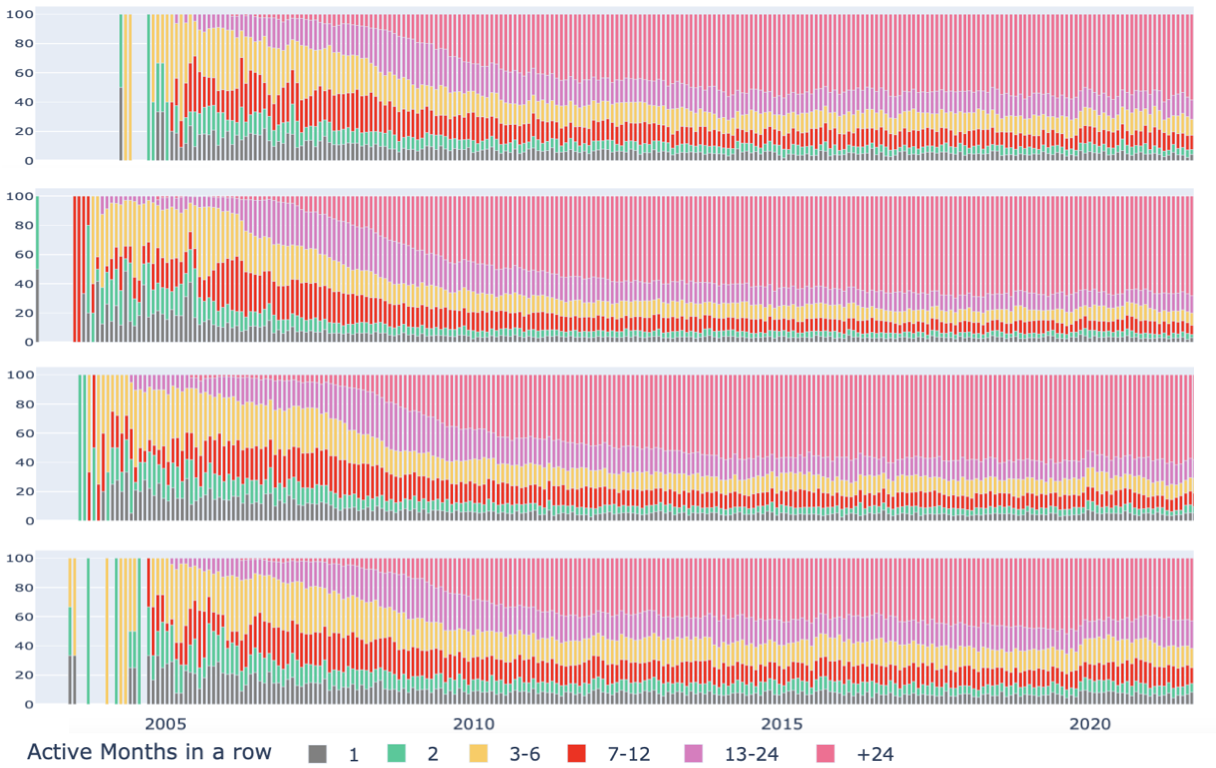
\includegraphics[width=480px]{img/stability_trend_v.png}
    \setlocalecaption{english}{figure}{Figure}
    \caption{Trend of the major European languages' stability among very active editors}
    \label{fig:stability_trend_v}
\end{figure}

While among the very active editors, the main part is represented by the editors which keep editing for more than 24 months. Since being a very active editor requires more effort than being simply active, we could argue that this very same effort pushes the editors towards being more and more dedicated to their role.\\
Ideally both fresh and long-term engaged editors should be present in every community.

\section{Balance}
\label{sec:balance_conclusion}

We now consider the balance visualizations. The Community balance metric measures the ability to maintain an equal proportion of old and new contributors.\\

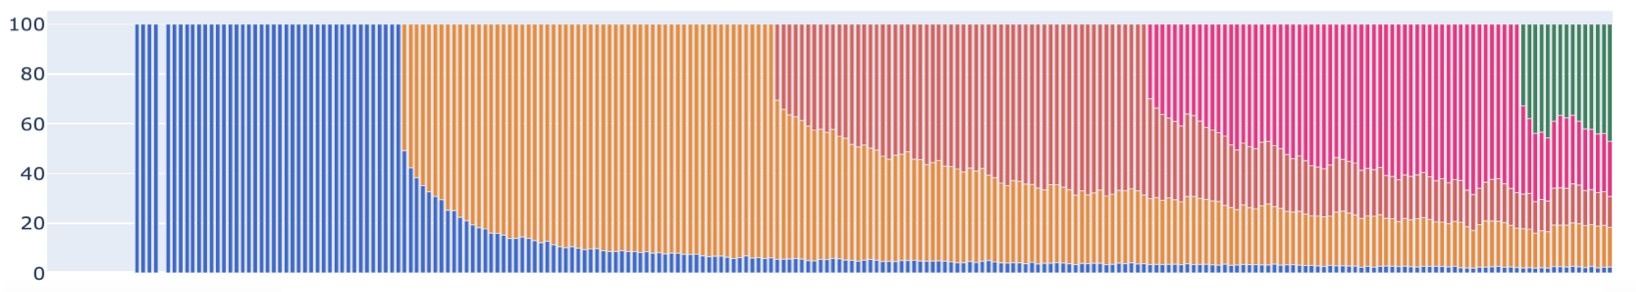
\includegraphics[width=470px]{img/balance_trend.png}
\pagebreak
\begin{figure}[h]
    \centering
    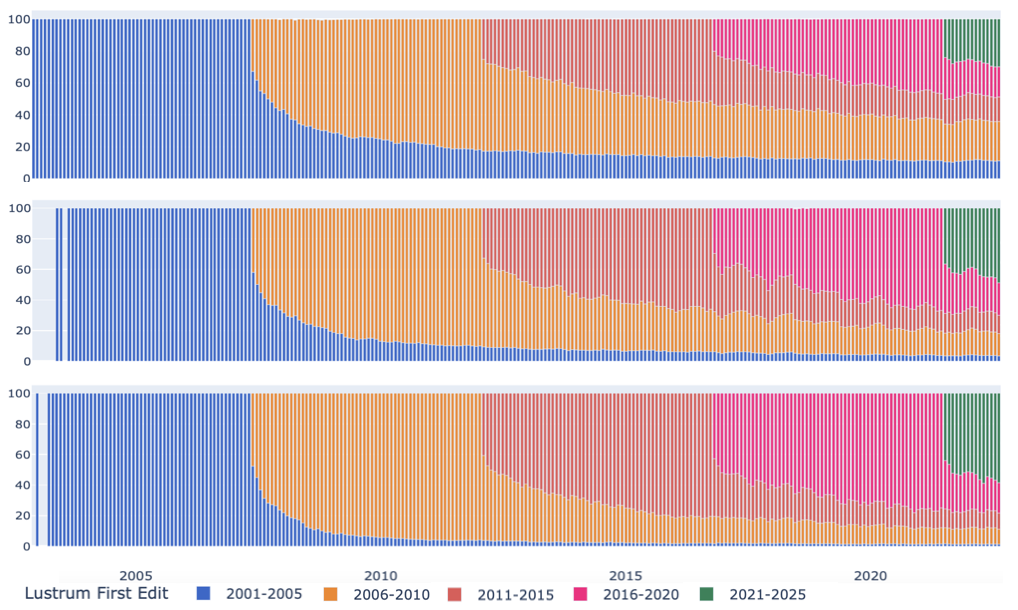
\includegraphics[width=470px]{img/balance_trend1.png}
    \setlocalecaption{english}{figure}{Figure}
    \caption{Trend of the major European languages' balance among active editors}
    \label{fig:balance_trend}
\end{figure}

In Figure \ref{fig:balance_trend} above we find, from top to bottom, Italian, German, French and Spanish.\\
There is a recurrent pattern: through the years, the new generations overtake the old ones, but not entirely. A generation is considered to be 5 years long.\\
The last generation (2021-2025) should occupy from 10 to 40\% depending on the years which have passed since its beginning, while the oldest generation (2001-2005) share should remain around 
5 to 15\%, not greater, to guarantee the generational change.

\section{Special functions}
\label{sec:special_conclusion}

Special functions are about editors which hold a certain role that allows them to perform special actions in Wikipedia. In particular, we have two distinct roles: Technical functions and Community coordination functions. We now analyze them both.

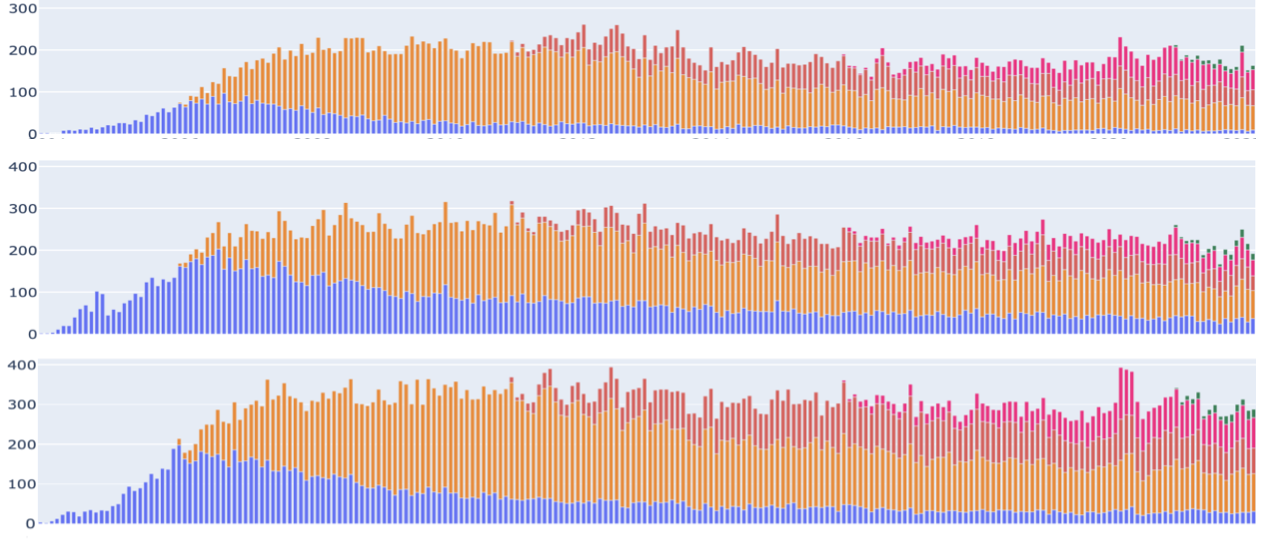
\includegraphics[width=470px]{img/tech_trend.png}
\begin{figure}[h]
    \centering
    
    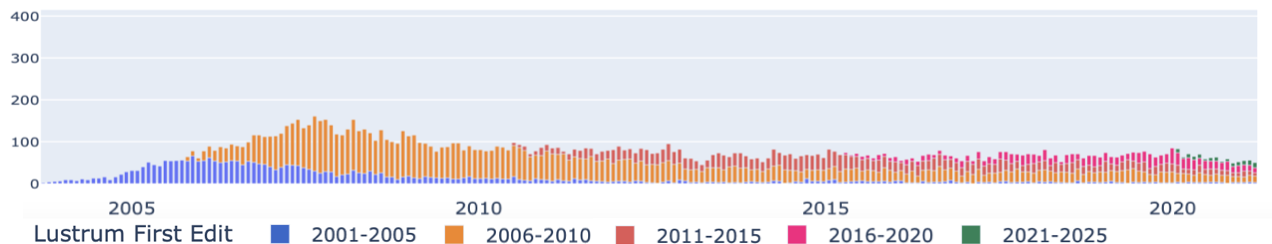
\includegraphics[width=470px]{img/tech_trend1.png}
    \setlocalecaption{english}{figure}{Figure}
    \caption{Trend of the major European languages' technical active editors}
    \label{fig:tech_trend}
\end{figure}
\pagebreak
\\
First we have technical editors. The majority of the them belongs to the 2006-2010 generation. The last generation 2021-2025 struggles at finding his space even if the older generation are now retreating.  From the Figure \ref{fig:tech_trend} we can clearly see that among active editors the color representing the second generation is significantly more present than the other generations. If we consult the online dashboards, we discover that, regardless of the editors being active or very active, this trend is consistent. Furthermore, it is a common pattern across different languages.

\begin{figure}[h]
    \centering
    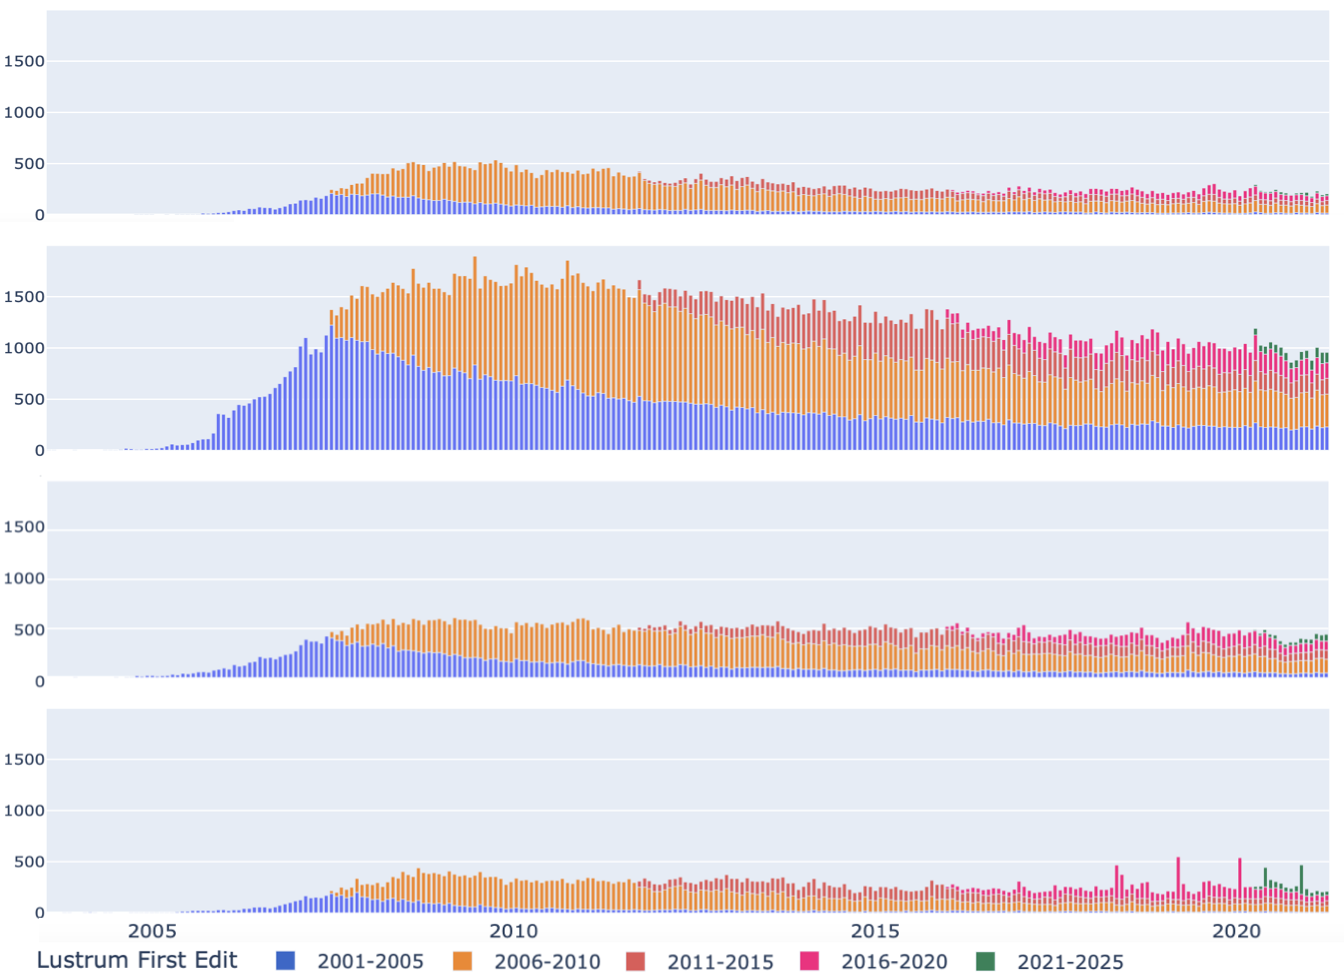
\includegraphics[width=470px]{img/coord_trend.png}
    \setlocalecaption{english}{figure}{Figure}
    \caption{Trend of the major European languages' coordinator active editors}
    \label{fig:coord_trend}
\end{figure}

Then we talk about coordinators. There are fewer and fewer new coordinators. As shown before when discussing technical editors, this trend is more evident among active editors visualizations, as we can see the color representing the second generation is more present than the other.\\
These trends could be the symptoms of a lesser interest in the specific functions of Wikipedia from the editors.\\
As before, we recommend to consult the online dashboard for a visualization taking in account both type of editors.

\section{Admin flags}
\label{sec:admin_conclusion}

We now observe the admin flags distribution among our language sample. This time the result is independent from the type of editors because it is function-specific. For this example, we only consider the ``sysop" flag since it is the most paradigmatic one among the admin flags.

\begin{figure}[h]
    \centering
    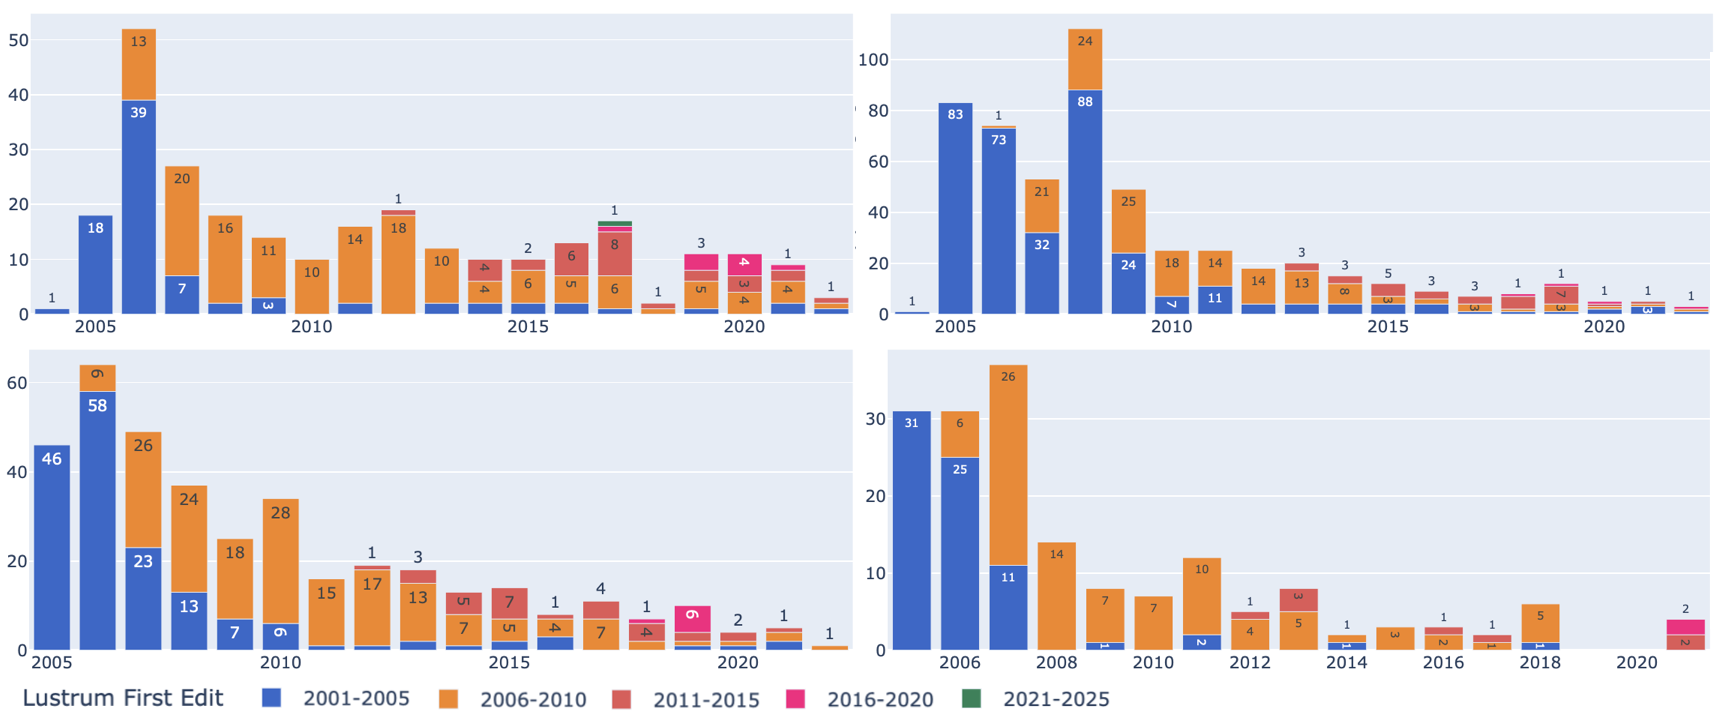
\includegraphics[width=470px]{img/admin_trend.png}
    \setlocalecaption{english}{figure}{Figure}
    \caption{Trend of the major European languages' admin distribution}
    \label{fig:admin_trend}
\end{figure}

In clockwise order we find Italian, German, Spanish and French.\\
Admin flags were given mainly in the past, especially to the first and second generation's editors.\\
In general, the percentage of a given admin flag, among active and very active editors, is borderline between being below and inline with the desired target of 1-5\%.

\section{Global community participation}
\label{sec:global_conclusion}

Finally we discuss the trend emerging from the global community. These trends are as important as the others since they move the focus on the bigger picture regarding the Wikipedia project as a whole. \\

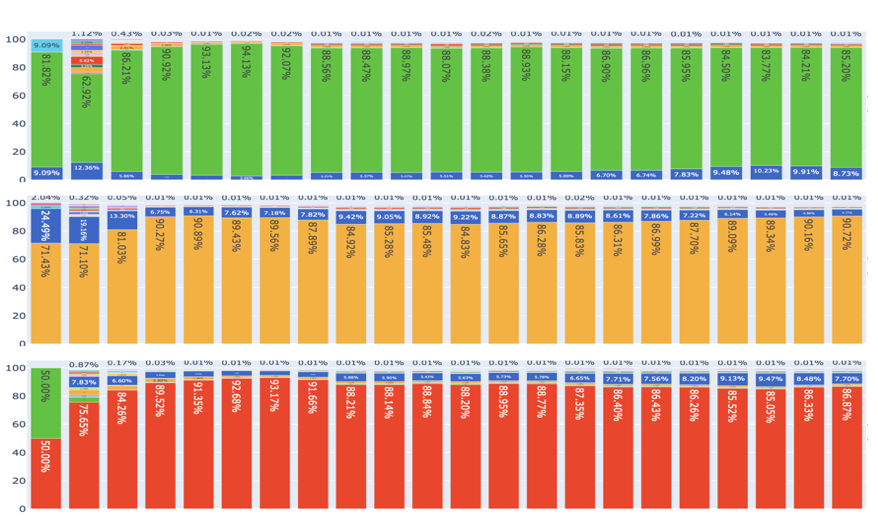
\includegraphics[width=470px]{img/global_trend.png}
\pagebreak
\begin{figure}[h]
    \centering
    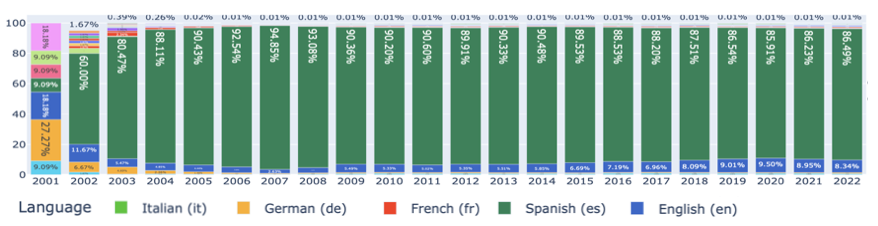
\includegraphics[width=470px]{img/global_trend1.png}
    \setlocalecaption{english}{figure}{Figure}
    \caption{Trend of the major European languages' global contribution}
    \label{fig:global_trend}
\end{figure}

From Figure \ref{fig:global_trend}, this time with a yearly time aggregation, we can see that the majority of the contributions for a given community come mainly from their primary language editors. In fact, the higher percentage has the same color of the analyzed language. However, the English community contributes consistently to every analyzed language. \\
We can observe a stabilizing trend: considering Italian and Spanish Wikipedia, in their early days they had different contributors that were, in percentage, much more active than today. Over the years, the minor communities percentage contribution decreased drastically, due to the affirmation of the big language community like German and English Wikipedia. Thus we can conclude that we lost diversity in the global contributions.This trend is inevitable, but the WikiCHM projects recommend the small community to keep editing in order to preserve their role in the global community.

\begin{figure}[h]
    \centering
    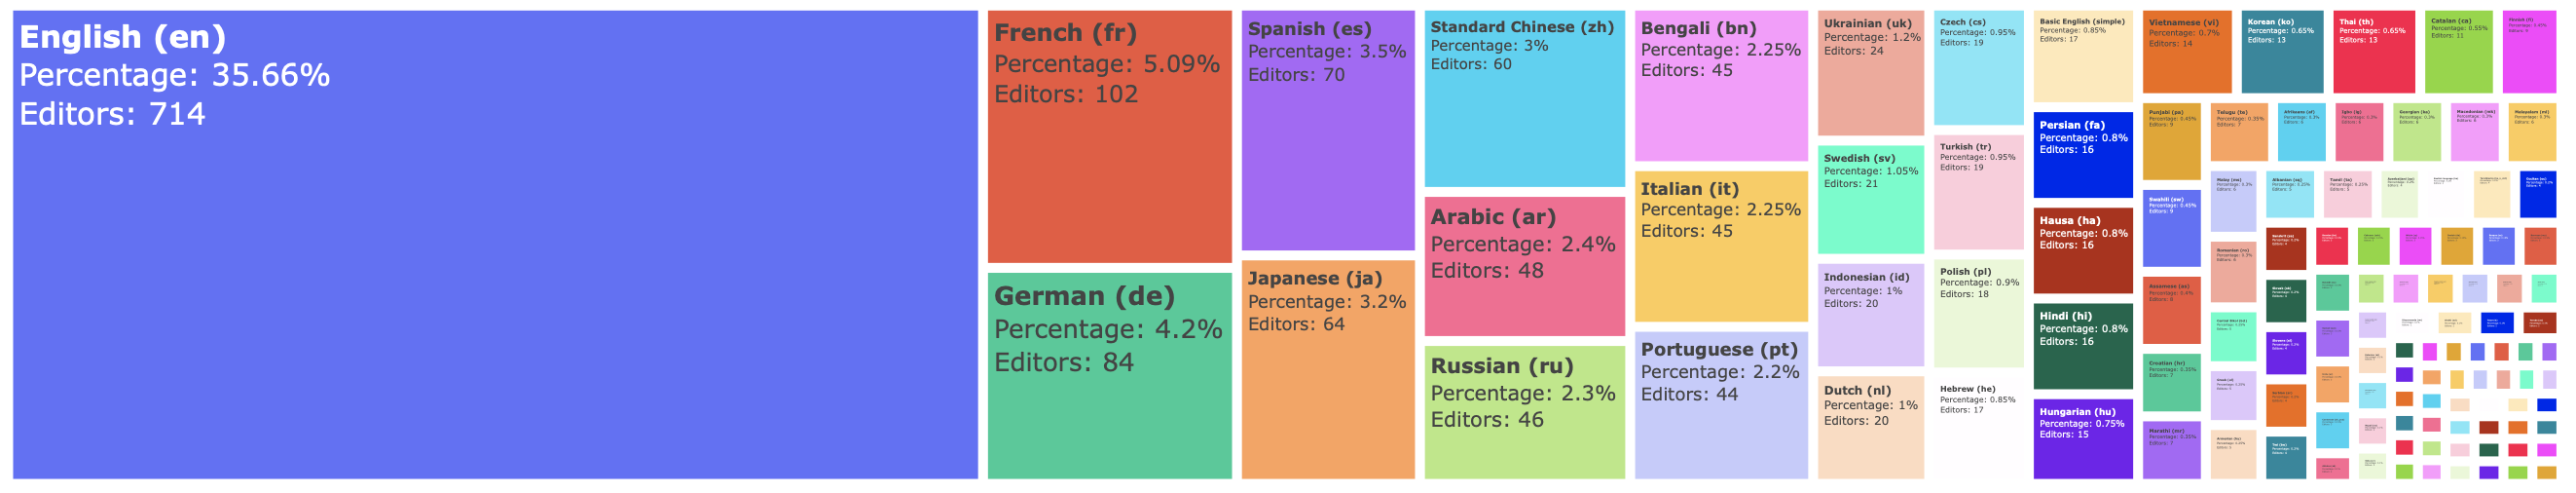
\includegraphics[width=470px]{img/meta_trend.png}
    \setlocalecaption{english}{figure}{Figure}
    \caption{Meta-wiki global participation }
    \label{fig:meta}
\end{figure}

Now we discuss the contribution of each language to the Meta-wiki. It is clear that the bigger language play a major role than the smaller ones. The English Wikipedia is the bigger contributor to the project, followed by other common languages like German, French but also Japanese and Chinese. \\
This result is extremely interesting since it shows that the European languages are not alone in the global Meta-wiki project, but there are the Asian giants too: the Japanese and Chinese community contributions reach, respectively, the 3.2\% and the 3\%; while the Arabic and Russian Wikipedia make their way among the big communities with, respectively, the 2.4\% and the 2.3\%.


      
      
    \endgroup


    % bibliografia in formato bibtex
    %
    % aggiunta del capitolo nell'indice
    \addcontentsline{toc}{chapter}{Bibliografia}
    % stile con ordinamento alfabetico in funzione degli autori
    \bibliographystyle{plain}
    \bibliography{biblio}
%%%%%%%%%%%%%%%%%%%%%%%%%%%%%%%%%%%%%%%%%%%%%%%%%%%%%%%%%%%%%%%%%%%%%%%%%%
%%%%%%%%%%%%%%%%%%%%%%%%%%%%%%%%%%%%%%%%%%%%%%%%%%%%%%%%%%%%%%%%%%%%%%%%%%
%% Nota
%%%%%%%%%%%%%%%%%%%%%%%%%%%%%%%%%%%%%%%%%%%%%%%%%%%%%%%%%%%%%%%%%%%%%%%%%%
%% Nella bibliografia devono essere riportati tutte le fonti consultate 
%% per lo svolgimento della tesi. La bibliografia deve essere redatta 
%% in ordine alfabetico sul cognome del primo autore. 
%% 
%% La forma della citazione bibliografica va inserita secondo la fonte utilizzata:
%% 
%% LIBRI
%% Cognome e iniziale del nome autore/autori, la data di edizione, titolo, casa editrice, eventuale numero dell’edizione. 
%% 
%% ARTICOLI DI RIVISTA
%% Cognome e iniziale del nome autore/autori, titolo articolo, titolo rivista, volume, numero, numero di pagine.
%% 
%% ARTICOLI DI CONFERENZA
%% Cognome e iniziale del nome autore/autori (anno), titolo articolo, titolo conferenza, luogo della conferenza (città e paese), date della conferenza, numero di pagine. 
%% 
%% SITOGRAFIA
%% La sitografia contiene un elenco di indirizzi Web consultati e disposti in ordine alfabetico. 
%% E’ necessario:
%%   Copiare la URL (l’indirizzo web) specifica della pagina consultata
%%   Se disponibile, indicare il cognome e nome dell’autore, il titolo ed eventuale sottotitolo del testo
%%   Se disponibile, inserire la data di ultima consultazione della risorsa (gg/mm/aaaa).    
%%%%%%%%%%%%%%%%%%%%%%%%%%%%%%%%%%%%%%%%%%%%%%%%%%%%%%%%%%%%%%%%%%%%%%%%%%
%%%%%%%%%%%%%%%%%%%%%%%%%%%%%%%%%%%%%%%%%%%%%%%%%%%%%%%%%%%%%%%%%%%%%%%%%%
    

    \titleformat{\chapter}
        {\normalfont\Huge\bfseries}{Allegato \thechapter}{1em}{}
    % sezione Allegati - opzionale
    \appendix
    \chapter{Titolo primo allegato}

Lorem ipsum dolor sit amet, consectetur adipiscing elit. Donec sed nunc orci. Aliquam nec nisl vitae sapien pulvinar dictum quis non urna. Suspendisse at dui a erat aliquam vestibulum. Quisque ultrices pellentesque pellentesque. Pellentesque egestas quam sed blandit tempus. Sed congue nec risus posuere euismod. Maecenas ut lacus id mauris sagittis egestas a eu dui. Class aptent taciti sociosqu ad litora torquent per conubia nostra, per inceptos himenaeos. Pellentesque at ultrices tellus. Ut eu purus eget sem iaculis ultricies sed non lorem. Curabitur gravida dui eget ex vestibulum venenatis. Phasellus gravida tellus velit, non eleifend justo lobortis eget. 

\section{Titolo}
Lorem ipsum dolor sit amet, consectetur adipiscing elit. Donec sed nunc orci. Aliquam nec nisl vitae sapien pulvinar dictum quis non urna. Suspendisse at dui a erat aliquam vestibulum. Quisque ultrices pellentesque pellentesque. Pellentesque egestas quam sed blandit tempus. Sed congue nec risus posuere euismod. Maecenas ut lacus id mauris sagittis egestas a eu dui. Class aptent taciti sociosqu ad litora torquent per conubia nostra, per inceptos himenaeos. Pellentesque at ultrices tellus. Ut eu purus eget sem iaculis ultricies sed non lorem. Curabitur gravida dui eget ex vestibulum venenatis. Phasellus gravida tellus velit, non eleifend justo lobortis eget. 

\subsection{Sottotitolo}
Lorem ipsum dolor sit amet, consectetur adipiscing elit. Donec sed nunc orci. Aliquam nec nisl vitae sapien pulvinar dictum quis non urna. Suspendisse at dui a erat aliquam vestibulum. Quisque ultrices pellentesque pellentesque. Pellentesque egestas quam sed blandit tempus. Sed congue nec risus posuere euismod. Maecenas ut lacus id mauris sagittis egestas a eu dui. Class aptent taciti sociosqu ad litora torquent per conubia nostra, per inceptos himenaeos. Pellentesque at ultrices tellus. Ut eu purus eget sem iaculis ultricies sed non lorem. Curabitur gravida dui eget ex vestibulum venenatis. Phasellus gravida tellus velit, non eleifend justo lobortis eget. 


\chapter{Titolo secondo allegato}

Lorem ipsum dolor sit amet, consectetur adipiscing elit. Donec sed nunc orci. Aliquam nec nisl vitae sapien pulvinar dictum quis non urna. Suspendisse at dui a erat aliquam vestibulum. Quisque ultrices pellentesque pellentesque. Pellentesque egestas quam sed blandit tempus. Sed congue nec risus posuere euismod. Maecenas ut lacus id mauris sagittis egestas a eu dui. Class aptent taciti sociosqu ad litora torquent per conubia nostra, per inceptos himenaeos. Pellentesque at ultrices tellus. Ut eu purus eget sem iaculis ultricies sed non lorem. Curabitur gravida dui eget ex vestibulum venenatis. Phasellus gravida tellus velit, non eleifend justo lobortis eget. 

\section{Titolo}
Lorem ipsum dolor sit amet, consectetur adipiscing elit. Donec sed nunc orci. Aliquam nec nisl vitae sapien pulvinar dictum quis non urna. Suspendisse at dui a erat aliquam vestibulum. Quisque ultrices pellentesque pellentesque. Pellentesque egestas quam sed blandit tempus. Sed congue nec risus posuere euismod. Maecenas ut lacus id mauris sagittis egestas a eu dui. Class aptent taciti sociosqu ad litora torquent per conubia nostra, per inceptos himenaeos. Pellentesque at ultrices tellus. Ut eu purus eget sem iaculis ultricies sed non lorem. Curabitur gravida dui eget ex vestibulum venenatis. Phasellus gravida tellus velit, non eleifend justo lobortis eget. 

\subsection{Sottotitolo}
Lorem ipsum dolor sit amet, consectetur adipiscing elit. Donec sed nunc orci. Aliquam nec nisl vitae sapien pulvinar dictum quis non urna. Suspendisse at dui a erat aliquam vestibulum. Quisque ultrices pellentesque pellentesque. Pellentesque egestas quam sed blandit tempus. Sed congue nec risus posuere euismod. Maecenas ut lacus id mauris sagittis egestas a eu dui. Class aptent taciti sociosqu ad litora torquent per conubia nostra, per inceptos himenaeos. Pellentesque at ultrices tellus. Ut eu purus eget sem iaculis ultricies sed non lorem. Curabitur gravida dui eget ex vestibulum venenatis. Phasellus gravida tellus velit, non eleifend justo lobortis eget. 




\end{document}
